\documentclass[AMA,STIX1COL]{WileyNJD-v2}

\articletype{Research Article}%

\received{26 April 2016}
\revised{6 June 2016}
\accepted{6 June 2016}

\raggedbottom

%% Below is my stuff

% Below are some packages for colors and graphics.
\usepackage{color}
\usepackage{graphicx}
\graphicspath{ {figures/} } %Setting the graphicspath
\usepackage{ifthen}
\usepackage{pdflscape}

% For tables
\usepackage{multirow}
\usepackage{booktabs}


%%%%% Keywords:
\newcommand{\Keywords}[1]{\par\noindent{\small{\em Keywords\/}: #1}}

\renewcommand{\vec}[1]{\mathbf{#1}}

%\DeclareMathOperator*{\argmin}{argmin}
\newcommand{\argmin}{\text{argmin}}
\newcommand{\diag}{\text{diag}}
\newcommand{\E}{\mathbb{E}}
\newcommand{\bd}[1]{\boldsymbol{#1}}
\newcommand{\Pn}{\mathbb{P}_{n}}


\begin{document}

\title{A simple framework to identify optimal risk thresholds for a single screen}


\author[1]{Hormuzd A. Katki*}
\author[2]{Ionut Bebu}

\authormark{Katki and Bebu}

\address[1]{\orgdiv{US National Cancer Institute}, \orgname{Division of Cancer Epidemiology and Genetics}, \orgaddress{\state{MD}, \country{USA}}}

\address[2]{\orgdiv{Biostatistics Center}, \orgname{George Washington University}, \orgaddress{\state{MD}, \country{USA}}}

\corres{*Hormuzd A. Katki, US National Cancer Institute, NIH, DHHS, 
	Division of Cancer Epidemiology and Genetics,
	9609 Medical Center Dr. Room 7E592 Rockville MD 20850. \email{katkih@mail.nih.gov}}

\presentaddress{US National Cancer Institute, NIH, DHHS, Division of Cancer Epidemiology and Genetics,
	9609 Medical Center Dr. Room 7E592 Rockville MD 20850}

%%% ----------------------------------------------------------------------
\setcounter{page}{1}   % begin to count from 1.
\pagenumbering{roman}   % assign the numbering system.

\setcounter{tocdepth}{3} % Set the depth of the contents.


%\tableofcontents
%\listoffigures % Have the list of figures.
%\listoftables % Have the list of tables.

\abstract[Summary]{ 
	Decision Curve Analysis (DCA) is a modern popular approach to identify the range of risk thresholds at which screening with a biomarker is the best decision.  However DCA does not directly account for costs and effectiveness of subsequent interventions, most applications assume a costless screening biomarker for simplicity, and DCA cannot formally identify optimal risk thresholds.  Although a full decision analysis can identify optimal risk thresholds, typically used methods are complex and it can be difficult to understand why they arrive at their conclusion.  We develop a simple framework to  calculate the Incremental Net Benefit (INB) for a single-time screen as a function of costs (screening test, definitive confirmatory test, and subsequent interventions) and effectiveness (dollar value of life-years gained by undergoing interventions).  We provide simple expressions for the optimal cost-effective risk-threshold and for the dollars per life-year gained threshold associated with an optimal risk-threshold.  We apply our framework to the controversy over the risk threshold for using the BRCAPRO risk model to screen women for mutations in \textit{BRCA1/2} that cause high risks of breast and ovarian cancers.  Our simple framework readily identifies sensitivity of DCA to biomarker test costs that is hard to see by DCA alone.  Importantly, most, and sometimes even all, of the optimal risk thresholds identified by DCA were infeasible based on their associated dollars per life-year gained threshold.  Our approach to estimating optimal risk thresholds in simple and transparent manner, providing intuition about which quantities are critical, may serve as a bridge between DCA and a full decision analysis.
	
	 %Mutations are rare in the general population, but more common among Ashkenazi-Jews. According to DCA, assuming costless BRCAPRO, optimal risk thresholds from 1\%-30\% support using BRCAPRO to screen among Ashkenazi-Jews.  However, our framework shows that all of these optimal risk-thresholds are infeasible because they imply a negative dollars per life-year gained threshold.  Furthermore, DCA is sensitive to a small cost of shared decision-making with BRCAPRO, which is hard to detect by DCA but easily seen by INB.    In the general population, optimal risk thresholds from 0.12\% to 0.91\% support screening.  However, these optimal thresholds represent dollars per life-year gained thresholds of \$16,000 to \$306,000, suggesting that none or only some of the optimal thresholds are feasible in practice, where thresholds below \$100,000 are typical.  
}

\keywords{AUC; \textit{BRCA1}; \textit{BRCA2}; cost effectiveness; decision analysis; Decision Curves; Diagnostic Testing; Incremental Net Benefit; Net Benefit; risk prediction ; ROC; Screening; Youden's index}

%	\jnlcitation{\cname{%
%			\author{Katki H.A.}} (\cyear{2018}), 
%		\ctitle{A regime analysis of Atlantic winter jet variability applied to evaluate HadGEM3-GC2}, \cjournal{Q.J.R. Meteorol. Soc.}, \cvol{2017;00:1--6}.}

\maketitle

%	\footnotetext{\textbf{Abbreviations:} ANA, anti-nuclear antibodies; APC, antigen-presenting cells; IRF, interferon regulatory factor}





%%%%%%%%%%%%%%%%%%%%%%%%%%%%%%%%%%%%%%%%%%%%%%%%%%%%%%%%%%%%%%%%%%%%%%%%%%
%%%%%%%%%%%%%%%%%%%%%%%%%%%%%%%%%%%%%%%%%%%%%%%%%%%%%%%%%%%%%%%%%%%%%%%%%%

% https://mdm.uic.edu/manuscript-requirements/

% REMOVE THE WORD DOLLAR IF SUBMIT TO NON-US JOURNAL!

\section{Introduction}
\label{sec:intro}
In population disease screening, a cheap, non-invasive, but imperfect test is conducted on a population to determine who should be referred for tests that are definitive for the presence of disease.   Because screening tests are imperfect indicators of the presence of disease, the goal is choose a screening test threshold that is cost-effective at controlling the rates of false classification.  There is much literature on identifying cost-effective thresholds~\citep{Pauker1980,Gail2005,Baker2009a}.  The cost-effective threshold requires specifying the costs, benefits, and harms of the tests and subsequent interventions.  However, statistical metrics that do not require costs, benefits, and harms, such as Youden's index, AUC, and Mean Risk Stratification~\citep{Katki2019}, cannot identify cost-effective thresholds.  

The most important recent advance is Decision Curve Analysis (DCA)~\citep{Vickers2006}.  DCA takes an important step towards formal decision analysis, but stops short of requiring specification of costs and effectiveness.  DCA is often used to identify a range of optimal risk-thresholds for using a risk-model to decide who should get intervention. However, there are two limitations of DCA.  First, most researchers in practice use DCA by assuming costless risk models. However, most risk models are not costless, typically requiring shared decision-making with a health professional.  DCA can acount for screening test costs, but this requires specification of costs and effectiveness and thus negates the simplicity of DCA.  More importantly, because DCA does not require costs and effectiveness, DCA considers risk-thresholds only as a sensitivity analysis and thus cannot formally identify optimal thresholds.

In contrast, a full decision analysis, specifying costs, benefits, and the monetary value of life, can determine cost-effective thresholds.  Often these analyses require complex decision trees and microsimulation.  It can be hard to glean intuition about which quantities and modeling assumptions are critical, even when probabilistic sensitivity analysis is conducted.  We suggest that there is a role for methodology for estimating optimal risk thresholds in simple and transparent manner, providing intuition about which quantities are critical, as a bridge between DCA and a full decision analysis.   

We propose a simple framework that identifies the cost-effective risk threshold for a single-time screen, such as screening for gestational diabetes, syphilis in pregnancy, or genetic mutations.   We calculate the Incremental Net Benefit (INB) based on specifying costs (screening test, definitive confirmatory test, and subsequent interventions) and effectiveness (dollar value of life-years gained by undergoing interventions).  We provide a simple expression for the optimal risk-threshold for the screening test that depends on only the cost of the definitive test and a parameter we call the net effectiveness of early intervention (NE).  Because the dollar-value of life-years gained is often hard to specify, we also provide an expression for the dollar-value of life-years gained implicitly implied by an optimal risk-threshold.

We apply our framework to the controversy over the risk-threshold to identify who should get testing for mutations in the \textit{BRCA1/2} genes, which cause high risks of breast and ovarian cancer~\citep{Kuchenbaecker2017}.   Current US and UK guidelines refer women for mutation testing only if they have a strong family history of breast or ovarian cancer~\citep{Moyer2014}, as quantified by a risk model calculating that their risk of carrying a \textit{BRCA1/2} mutation exceeds 10\%~\citep{NICE2017}.  However, as mutation-testing costs plummet, prominent voices have called for testing \textit{all} women~\citep{King2014}, equivalent to a 0\% risk-threshold.   The Screen Project offers \textit{BRCA1/2} testing to any Canadian~\citep{TheScreenProject2017}.  In a landmark ruling, the US FDA authorized direct-to-consumer genetic testing for \textit{BRCA1/2} mutations among Ashkenazi-Jews~\citep{Rabin2018}.  %Population mutation screening is inevitable, but there are strong disagreements on how such programs should be conducted.

We recently showed that 80\% of Ashkenazi-Jewish mutation-carriers could be identified by testing only 44\% of Ashkenazi-Jewish women at highest risk for carrying mutations~\citep{Best2019}, as identified by the BRCAPRO risk model~\citep{Parmigiani1998}.  This is achieved by a low mutation-risk threshold of 0.78\%, far lower than the current 10\% US and UK guideline.  We previously examined multiple statistical metrics, such as AUC, DCA, and Mean Risk Stratification~\citep{Katki2019}, to examine properties of different risk thresholds.  However, no statistical metric can formally identify optimal cost-effective risk-thresholds.  In this paper, we input costs and benefits into our simple framework to identify optimal risk thresholds to screen women for referral for \textit{BRCA1/2} genetic testing.  In this example, we show that DCA is sensitive to the standard assumption of a costless screening test, but this is hard to see by DCA.  Our framework easily identifies this sensitivity.  More importantly, many, or even sometimes all, the risk thresholds identified by DCA as being favorable for screening implied unfeasible values of dollars per life-year gained.  Our results are comparable to those from more comprehensive microsimulation-based decision analyses, while retaining the benefits of simplicity, transparency, and ease of identifying the critical quantities that the decision analysis is sensitive to.



%For Ashkenazi-Jews, the range of risk thresholds identified by Net Benefit as favoring screening is misleading because the dollars per life-year gained implied by these thresholds is negative and thus not allowable.  This means that performing BRCA1/2 genetic testing on all Ashkenazi-Jewish women would save money versus using BRCAPRO to screen to identify who should get genetic testing.

%Using our simple framework, our findings are comparable to more comprehensive, but more complex and less transparent, microsimulation approaches to this issue~\cite{Long2015,Manchanda2015}.  

%This is the basis for recent developments in risk prediction metrics, such as Net Benefit.  In current approaches, the utilities are left unspecified and all possible risk thresholds are considered as a sensitivity analysis.  Because costs, benefits and harms require specification, we propose that scientists who evaluate new medical tests or propose thresholds for test must try to specify these as best as possible.  

\section{A cost-effectiveness framework for a single-time screen}

The goal of a single-time screen is to identify all cases of prevalent disease for early detection and treatment.  Although disease could be absent at the time of screen and develop later, that requires longitudinal screening to detect, which is beyond the scope of this paper.  Thus the goal of a single-screen is solely to mitigate the impact of disease that is currently present by detecting it early for immediate treatment, rather than detecting it later when treatment may be less effective.  This framework includes both detecting disease early when it is curable (i.e. early detection) and detecting disease in a precursor state where its removal prevents future potentially incurable disease (i.e. secondary prevention). 

\subsection{Defining average costs and effectiveness for a single-time screen} 
\label{sec:framework}

In screening, asymptomatic people are given the single screening test.  Two outcomes are possible.  The first outcome is a positive test, after which a person is referred for definitive disease testing.  If disease is diagnosed, it is then treated.  Because the screening test found the disease early (i.e. in the absence of symptoms), presumably treatment is more effective than for disease found later on the basis of symptoms.

The second outcome is that the test is negative, after which there is no further action.  However, future symptoms will prompt definitive testing to diagnose disease that was present but missed by the screen.  If disease were diagnosed in the future based on symptoms, then presumably treatment is less effective (or most costly) than it would have been had disease been found earlier.

\noindent Four parameters define the average costs for a single screen:  

First is $c_m$, the cost of screening marker evaluation.  Note that the screening test is imperfect, else it would be the definitive test.  The main goal of our paper is to identify the cost-effective threshold for deciding screening test positivity.  

Second is $c_0$, the cost of the definitive test for disease, e.g. biopsy or imaging.  We presume this test is perfect but is so invasive or costly that, practically, it cannot be the screening test.  

Third is $c_1$, the cost of treatment for a disease case diagnosed early.  This occurs for those testing positive for disease on both the screening test and definitive test.  

Fourth is $c_2$, the treatment cost for a disease case diagnosed late.  This occurs for those with negative screening test (or not screened at all), but in the future develop symptoms and disease is diagnosed by the definitive test.
\newline
\newline
\noindent  Three parameters define the average effectiveness of a single screen, defining effectiveness as life-expectancy:  

First is $e_0$, the life-expectancy for someone who never develops disease.  This is assumed to be the same for those who correctly tested negative or falsely tested positive for the single screening test.

Second is $e_1$, the life-expectancy for someone who screens positive and the definitive test is also positive for disease.  This is early-detection and is the benefit of screening.  

Third is $e_2$, the life-expectancy for someone who is either not screened or tests screen-negative, but then develops disease.  This is late detection and is a screening failure.  We presume that $e_1 \ge e_2$, else screening causes obvious harm. 

%In section~\ref{sec:SensAnaly}, we examine sensitivity to specification of costs and effectiveness.  In the Discussion, we consider practical weaknesses of our approach to identifying costs and effectiveness.

\subsection{Calculating Net Benefit (NB)}
\label{sec:INB}

%The INB is the difference in average costs and effectiveness of a 1-time screen versus never screening.  

Define disease as $D$ and the marker for the screening test as $M$.   The marker is dichotomized as positive ($M+$) or negative ($M-$) based on a underlying threshold $m_0$ (our goal will be to identify the cost-effective $m_0$).  The components of the average cost and effectiveness are:
\begin{enumerate}
			\item{True Positive: The screening is positive and the individual has disease ($M+,D+$). \\ Cost is $c_m+c_0+c_1$ and effectiveness is $e_1$.}
			\item{False Positive: The screening is positive but the individual does not have disease ($M+,D-$).  \\ Cost is $c_m+c_0$ and effectiveness is $e_0$.}
			\item{False Negative: The screening is negative but the individual has disease ($M-,D+$).  \\Cost is $c_m+c_0+c_2$ and effectiveness is $e_2$.}
			\item{True Negative: The screening is negative and the individual does not have disease ($M-,D-$).  \\ Cost is $c_m$ and effectiveness is $e_0$.}
\end{enumerate}
Let $C_M$ and $E_M$ be the average cost and effectiveness for screening, respectively, so that:
\begin{eqnarray*}
	{\cal E} (C_M) &=& c_m + [1-P(D-,M-)]\cdot c_0+P(D+,M-)\cdot c_2+P(D+,M+)\cdot c_1\\
	{\cal E} (E_M) &=& e_0\cdot P(D-) + P(D+,M+)\cdot e_1 + P(D+,M-)\cdot e_2,
\end{eqnarray*}
where ${\cal E(X)}$ represents the expected value of random variable $X$.  The Net Benefit (NB) is the difference of average effectiveness and cost for screening:
\begin{eqnarray}
	\label{eq:NB_M}
	N\!B_{M} &=& {\cal E} (\lambda E_M-C_M) \nonumber \\
				  &=&\lambda e_0P(D-) - c_m - c_0P(D-,M+) + (\lambda e_1-c_0-c_1)P(D+,M+) + (\lambda e_2-c_0-c_2)P(D+,M-),
\end{eqnarray}
where $\lambda$ is the "willingness to pay parameter" that measures the dollar-value of 1 year of life.

%The differences in cost and effectiveness between screening and never screening are:
%\begin{eqnarray*}
%	\Delta C &=& c_m + c_0\cdot P(M+) + (c_1 - c_2 - c_0)\cdot P(D+,M+)\\
%	\Delta E &=& d(e_1 - e_2)\cdot P(D+,M+).
%\end{eqnarray*}
%
%\noindent The Incremental Net Benefit is
%\begin{eqnarray} 
%I\!N\!B &=& \Delta E - \Delta C\\ \nonumber
%&=& [d(e_1-e_2)-(c_1-c_2-c_0)]P(D+,M+) - c_m - c_0P(M+)\\ \nonumber
%&=& [e+c_0]P(D+,M+) - c_m - c_0P(M+), \label{eq:INB}
%\end{eqnarray}
%where $e = d(e_1-e_2)-(c_1-c_2)$ is the "net effectiveness of early intervention". The net effectiveness contrasts the dollar-value of the life-expectancy gain with dollar increase in treatment cost for early vs. late detection.  If net effectiveness $e<0$, screening is never cost-effective (See WebAppendix).   Life-expectancy in the absence of disease ($e_0$) is not needed.

%The INB reveals that only certain aspects of costs and effectiveness require specification. First, only the dollar-value of life-years gained $d(e_1-e_2)$ requires specification.  Life-expectancy in the absence of disease ($e_0$) is not needed.  Second, only the difference of early vs. late treatment costs $c_1-c_2$ requires specification.  

%Importantly, if treatment costs were similar regardless of early versus late detection, or if treatment costs are far below the dollar value of life-years gained, then net effectiveness approximately depends only only the value of life-years gained.


\subsection{Optimal cost-effective risk threshold that maximizes the Net Benefit of screening}
\label{sec:optimalthreshold}

Given a screening marker or risk model $M$, a screening test is declared either $M+=\{M \ge m_0\}$ as positive or $M-=\{M<m_0\}$ as negative. Assume that $M$ is unbiased, meaning $P(D+|M=m) = m$.  We derive the optimal threshold $m_0$ that maximizes the Net Benefit of screening.  Let $f_M$ denote the density of $M$, so that
\begin{eqnarray*} \nonumber
	P(D+,M+) &=& \int_{m_0}^\infty P(D+|M=m) f_M(m)\,dm = \int_{m_0}^\infty m f_M(m)\,dm \\	
	P(D-,M+) &=& \int_{m_0}^\infty P(D-|M=m) f_M(m)\,dm = \int_{m_0}^\infty (1-m)f_M(m)\,dm \\
	P(D+,M-) &=& P(D+)-P(D+,M+) = P(D+) - \int_{m_0}^\infty m f_M(m)\,dm.
\end{eqnarray*}
Plugging the above into the Net Benefit for screening $N\!B_M$ yields
\begin{eqnarray*}
	N\!B_M &=& \lambda e_0P(D-) - c_m - c_0 \int_{m_0}^\infty (1-m) f_M(m)\,dm + (\lambda e_1-c_0-c_1)\int_{m_0}^\infty m f_M(m)\,dm + (\lambda e_2-c_0-c_2)\left( P(D+) - \int_{m_0}^\infty m f_M(m)\,dm \right).
\end{eqnarray*}
Taking the derivative of $N\!B_M$ with respect to $m_0$ and setting it equal to zero yields
\begin{eqnarray*}
	c_0(1-m_0)f_M(m_0) - (\lambda e_1-c_0-c_1)m_0f_M(m_0) + (\lambda e_2-c_0-c_2)m_0f_M(m_0)= 0.
\end{eqnarray*}
Solving for $m_0$ yields the optimal cost-effective risk threshold, denoted $R(\lambda)$, that maximizes the Net Benefit of screening:
\begin{eqnarray}
	\label{eq:R}
	m_0 = \frac{c_0}{e(\lambda)+c_0} \equiv R(\lambda),
\end{eqnarray}
where $e(\lambda)=\lambda(e_1-e_2)-(c_1-c_2)$ is the "net effectiveness of early intervention". The net effectiveness $e(\lambda)$ contrasts the dollar-value of the life-expectancy gain with dollar increase in treatment cost for early vs. late detection.  If $e(\lambda)<0$, then optimal threshold $R(\lambda)$ does not exist.  We emphasize that $e(\lambda)$, and hence optimal threshold $R(\lambda)$, is a function of the willingness-to-pay parameter $\lambda$, which varies between people and populations.  We will vary $\lambda$ in our examples.

The optimal threshold $R(\lambda)$ requires specification of only the definitive test cost $c_0$ and the net effectiveness of early intervention $e(\lambda)$.  Life-expectancy in the absence of disease ($e_0$) is not needed.  Also the screening test cost $c_m$ is not needed, because risk thresholds only matter after the screening test is conducted, and thus the screening test cost is a sunk cost.  However, $e_0$ and screening test cost will matter to check whether optimal screening is cost-effective (Section~\ref{sec:INBgain}).  %In the following examples, we obtain $c_0$ and $e(\lambda)$ from data (varying $\lambda$) to directly propose optimal thresholds.

Defining $M_R+=\{M \ge R(\lambda)\}$ and $M_R-=\{M<R(\lambda)\}$, we denote the Net Benefit of screening with the optimal $R$ as
\begin{eqnarray}
\label{eq:NB_M(R)}
N\!B_{M}(R) &=& \lambda e_0P(D-) - c_m - c_0P(D-,M_R+) + (\lambda e_1-c_0-c_1)P(D+,M_R+) + (\lambda e_2-c_0-c_2)P(D+,M_R-).
\end{eqnarray}
The notation $M_R+$ and $M_R-$ clarifies that marker/model must be dichotomized at the optimal threshold $R(\lambda)$.
 
The WebAppendix derives the optimal threshold $R$ from the classical expected utility approach~\citep{Pauker1980}.

%Neither screening test characteristics nor disease prevalence matter for calculating the optimal risk-threshold.  This is unlike metrics such as MRS, Youden's index, AUC, Vickers's Net Benefit gain, which are all maximized at risk threshold equals disease prevalence (i.e $m_0=P(D+)$), regardless of costs and effectiveness~\citep{Katki2019}. 
% Derivation of optimal risk threshold for the INB of screening vs. testing no one:
%\begin{equation*}\label{risk_model}
%	P(D+|M=m) = m  \,.
%\end{equation*}
%Let $f_M$ denote the density of $M$, and denote the  threshold $m_0$, so that
%\begin{eqnarray*} \nonumber
%	P(M+) &=& \int_{m_0}^\infty f_M(m)\,dm\\  \label{expressions}
%	P(D+,M+) &=& \int_{m_0}^\infty P(D+|M=m)\cdot f_M(m)\,dm\\   \nonumber
%	&=& \int_{m_0}^\infty m\cdot f_M(m)\,dm\,.
%\end{eqnarray*}
%INB can be writen as 
%\begin{equation*}\label{INB2}
%	INB=(e+c_0)\cdot \int_{m_0}^\infty m\cdot f_M(m)\,dm - c_0\cdot \int_{m_0}^\infty f_M(m)\,dm - c_m\,.
%\end{equation*}
%Taking the derivative with respect to $m_0$ and setting it to zero yields
%\[-(e+c_0)\cdot m_0\cdot f_M(m_0) + c_0\cdot f_M(m_0) =0\,, \]
%Thus the optimal risk threshold maximixing INB is:
%\begin{eqnarray*}
%	m_0 = \frac{c_0}{e+c_0}. 
%\end{eqnarray*}

\subsubsection{Willingness-to-pay $\lambda$ implied by optimal risk-thresholds}
\label{sec:DollarsPerLYG}

Because the willingness-to-pay $\lambda$ for 1-year of life varies between people and populations, is difficult to specify the optimal $R(\lambda)$. Thus some analyses, such as Decision Curve Analysis\cite{Vickers2006}, vary $R(\lambda)$ as a sensitivity analysis, without regard to $\lambda$.  However, there is a one-to-one relationship of $R(\lambda)$and $\lambda$ (equation~\ref{eq:R}), and thus a given $R(\lambda)$ may not be feasible in practice its corresponding $\lambda$ is not realisitic.  For example, if a particular optimal $R(\lambda)$ required valuing 1 year of life at $\lambda=\$1$ million USD, then that optimal threshold is not feasible in practice because typically $\lambda\le\$100,000$ USD.  Solving for $\lambda$ in equation~\ref{eq:R} yields
\begin{eqnarray}
\label{eq:dollarsperLYG}
\lambda(R) &=& \frac{c_0(1-R)/R + (c_1-c_2)}{e_1-e_2}.
\end{eqnarray}
An optimal risk threshold $R(\lambda)$, fixing costs and life-years gained, implies a unique willingness-to-pay $\lambda(R)$.  In analyses where the optimal risk threshold is varied, as in our example or Decision Curve Analysis\cite{Vickers2006}, one needs to also calculate the $\lambda(R)$ underlying the optimal risk threshold $R(\lambda)$ to see if $R(\lambda)$ is a feasible threshold.  
 
%This expression is key to understanding if an optimal risk-threshold implies a feasible value of dollars per life-year gained.

\subsection{Incremental Net Benefit versus screening no one or testing everyone}
\label{sec:INBgain}
In addition to screening with the optimal threshold $R$, two other policies are possible:  test no one, or do definitive testing on everyone.  To ensure that Net Benefit from screening with the optimal threshold $R$ (equation~\ref{eq:NB_M(R)}) is the best policy, we must compare to the Net Benefits of the other two policies.

For testing no one, if the person has disease ($D+$), then cost is $c_0+c_2$ and effectiveness is $e_2$.  If the person does not have disease ($D-$), then cost is 0 and effectiveness is $e_0$.  The Net Benefit of testing no one is $N\!B_{none} = \lambda e_0P(D-)+ (\lambda e_2-c_0-c_2)P(D+)$.  For testing everyone, if the person has disease ($D+$), then the cost is $c_0+c_1$ and effectiveness is $e_1$.  If the person does not have disease ($D-$), then cost is $c_0$, effectiveness is $e_0$.  The Net Benefit of testing everyone is 
$N\!B_{all} = (\lambda e_0-c_0)P(D-) + (\lambda e_1-c_0-c_1)P(D+)$. 

To compare the 3 Net Benefits, we calculate the Incremental Net Benefit (INB) of screening vs. each of the other 2 policies:
\begin{eqnarray*}
	I\!N\!B_{none}(R) &=& N\!B_M(R)-N\!B_{none}~~\mathrm{and}~~ I\!N\!B_{all}(R) = N\!B_M(R)-N\!B_{all}.
\end{eqnarray*}

If both $I\!N\!B_{none}(R)>0$ and $I\!N\!B_{all}(R)>0$, then screening at optimal threshold $R$ is best. To summarize both conditions into a single condition, we define
\begin{eqnarray}
\label{eq:INB_Gain}
	I\!N\!B_{Gain}(R) &=& min(I\!N\!B_{none}(R),I\!N\!B_{all}(R)),	
	%I\!N\!B_{Gain}(R) &=& N\!B_M(R) - max(N\!B_{none},N\!B_{all}),
\end{eqnarray}
and require that $I\!N\!B_{Gain}(R)>0$ for screening at threshold $R$ to be the best policy.  Note that the threshold $R$ that maximizes $N\!B_M(R)$ (equation~\ref{eq:R}) also maximizes $I\!N\!B_{Gain}(R)$ because neither $N\!B_{none}$ nor $N\!B_{all}$ are functions of $R$.  Although optimal threshold $R$ is not a function of life-expectancy $e_0$ or screening test cost $c_m$, note that $N\!B_M(R)$ requires $c_m$, and both $N\!B_{none}$ and $N\!B_{all}$ require $e_0$, so that both $c_m$ and $e_0$ matter to check if optimal screening is superior to testing no one or testing everyone.

In the examples, we will use $I\!N\!B_{Gain}(R)$ to identify the range of optimal thresholds $R$ such that screening is the best policy.  Note that by varying optimal threshold $R(\lambda)$, but fixing costs and effectiveness, we are implicitly varying $\lambda$.   We will also plot $I\!N\!B_{Gain}(R)$ versus $\lambda(R)$ to understand if an optimal threshold implies a feasible willingness-to-pay $\lambda(R)$.

%If $I\!N\!B(R)>0$, then screening based on the marker is more cost-effective than screening no one.  To also check if screening is also more cost-effective than just conducting the definitive test on everyone, we have to compare the INB versus the INB for testing everyone versus screening no one, called $I\!N\!B_{all}$.   For testing everyone, we have $P(D+,M+)=P(D+)$, $P(M+)=1$, and $c_m=0$ since we don't need the screening test.  Plugging these into equation~\ref{eq:INB} yields $I\!N\!B_{all}=(e+c_0)P(D+)-c_0$.  The $I\!N\!B_{Gain}$ is the increase in INB beyond either screening no one or testing everyone:
%\begin{eqnarray}
%\label{eq:INBgain}
%I\!N\!B_{Gain}(R) = I\!N\!B(R) - max(0,I\!N\!B_{all}) = \{c_0P(D+,M+)/R - c_m - c_0P(M+)\} - max(0,c_0P(D+)/R-c_0),
%\end{eqnarray}
%by substituting the optimal risk threshold $R=c_0/(e+c_0)$.  Risk thesholds where $I\!N\!B_{Gain}(R)>0$ are thresholds where screening is better than screening no one or testing everyone.

%Let $C_{none}$ and $E_{none}$ be the average cost and effectiveness for testing no one, and $C_{all}$ and $E_{all}$ for testing everyone:
%\begin{eqnarray*}
%	{\cal E} (C_{none}) &=& (c_0+c_2)\cdot P(D+) \\
%	{\cal E} (E_{none}) &=& e_2\cdot P(D+) + e_0\cdot P(D-) \\
%	{\cal E} (C_{all}) &=& c_0 + c_1\cdot P(D+) \\
%	{\cal E} (E_{all}) &=& e_1\cdot P(D+) + e_0\cdot P(D-).
%\end{eqnarray*}




\subsubsection{Comparison of INB to Decision Curve Analysis}
\label{sec:NB}

Decision Curve Analysis (DCA) calculates a "Net Benefit (NB)" to identify risk thresholds where using a screening marker to decide who should get treated is better than treating no one or testing everyone~\citep{Vickers2006}.  We now show that the NB from DCA equals the $I\!N\!B_{none}$ divided by net effectiveness $e(\lambda)$.  Note that $I\!N\!B_{none}(R) = N\!B_M(R) - N\!B_{none}$ is
\begin{eqnarray*}
	I\!N\!B_{none}(R) &=& \{\lambda e_0P(D-) - c_m - c_0P(D-,M_R+) + (\lambda e_1-c_0-c_1)P(D+,M_R+) + (\lambda e_2-c_0-c_2)P(D+,M_R-)\} \\
	&&- \{\lambda e_0P(D-)+ (\lambda e_2-c_0-c_2)P(D+)\}\\
	&=& e(\lambda)P(D+,M_R+) - c_0P(D-,M_R+) - c_m.	
\end{eqnarray*}
The $I\!N\!B_{none}(R)$ divided by net effectiveness $e(\lambda)$ equals the Net Benefit from DCA, denoted $N\!B_{DCA}(R)$ as a function of $R$:
\begin{eqnarray*}
	N\!B_{DCA}(R) &=& \pi\cdot Sens-\frac{R}{1-R}(1-Spec)(1-\pi) - \frac{c_m}{e(\lambda)},
%	P(D+,M_R+)-\frac{R}{1-R}P(D-,M_R+) - \frac{c_m}{e(\lambda)} \\
\end{eqnarray*}				
where $c_0/e(\lambda) = R/(1-R)$, $\pi=P(D+)$, $Sens=P(M_R+|D+)$, and $Spec=P(M_R-|D-)$.\citep{Vickers2006}  Note that the marker/model must be dichotomized at the optimal threshold $R$.

DCA also must compare the $N\!B_{DCA}$ for screening versus the $N\!B_{DCA}$ of the two policies of testing no one or testing everyone.  To summarize both comparisons into a single condition akin to $I\!N\!B_{Gain}(R)$ of equation~\ref{eq:NB_Gain}, we define $N\!B_{Gain}(R)$ as increase in $N\!B_{DCA}(R)$ versus the $N\!B_{DCA}$ of the other 2 policies\cite{Katki2019}.  The $N\!B_{DCA}$ for testing no one is $(N\!B_{none} - N\!B_{none})/e(\lambda)=0$.  The $N\!B_{DCA}$ for testing everyone is $(N\!B_{all} - N\!B_{none})/e(\lambda)$.  Thus we define 
\begin{eqnarray*}
	N\!B_{Gain}(R) = N\!B_{DCA}(R) - max(0,(N\!B_{all} - N\!B_{none})/e(\lambda)).
%	N\!B_{Gain}(R) = N\!B(R) - max(0,I\!N\!B_{all}/e(\lambda)) = N\!B(R) - max(0,P(D+)/(1-R)-R).
\end{eqnarray*}
For a costless screening test $c_m=0$, $N\!B_{DCA}$ does not require specifying the net effectiveness $e(\lambda)$.  In this case, $N\!B_{DCA}$ is a function of only risk threshold $R$.  This is a major advantage of $N\!B_{DCA}$ in practice, allowing one to plot $N\!B_{DCA}$ as a function of $R$ to identify the range of risk thresholds supporting screening, without having to specify any cost or effectiveness parameters.  The thresholds $R$ where $N\!B_{Gain}(R)>0$ are thresholds where the risk model is better than screening no one or testing everyone.  In particular, $N\!B_{Gain}(R)$ is maximized at optimal risk threshold equals disease prevalence, $R=P(D+)$.~\cite{Katki2019}  If the risk threshold is below prevalence, then if $N\!B_{Gain}(R)<0$, then testing everyone is the favored policy.   If the risk threshold is above prevalence, then if $N\!B_{Gain}(R)<0$, then testing no one is the favored policy. 

These are the same thresholds as where $I\!N\!B_{Gain}(R)>0$.  However, using $I\!N\!B_{Gain}$ has 2 key advantages over the $N\!B_{Gain}(R)$ of DCA.  The first advantage of $I\!N\!B_{Gain}(R)>0$ is that one can examine if an optimal risk threshold $R(\lambda)$ is feasible by calculating the $\lambda$ underlying it (equation~\ref{eq:dollarsperLYG}).  Second, screening tests are not costless.  Even most risk models are not costless, requiring at least a patient's time to fill out inputs and to comprehend outputs, and usually requires a visit with a health professional.  Although it is straightforward to specify $c_m$, note that this then requires also specifying net effectiveness $e(\lambda)$ which requires costs and effectiveness.  Thus accounting for screening test cost in DCA also requires all the other costs and effectiveness, negating the key advantage of DCA as not requiring costs and effectiveness.    

%\subsection{INB versus testing everyone}
%\label{sec:INBvsAll}
%
%We must also compare screening versus conducting the definitive test on everyone in the population.  As noted in the introduction, this is relevant to genetic testing, where the costs of genetic testing is becoming so cheap that there are calls to simply test everyone.  Everyone undergoes definitive testing, but all prevalent disease is detected early:
%\begin{enumerate}
%	\item{The individual has disease ($D+$): cost is $c_0+c_1$ and effectiveness is $e_1$}
%	\item{The individual does not have disease ($D-$): cost is $c_1$, effectiveness is $e_0$.}
%\end{enumerate}
%Following the argument of section~\ref{sec:INB}, the INB comparing screening versus testing everyone is
%\begin{eqnarray}
%INB_{all} &=& -[e+c_0]P(D+,M-) - c_m + c_0P(M-).
%\end{eqnarray}
%For screening to be the best decision, both $INB>0$ and $INB_{all}>0$.


\section{Example: Who should undergo \textit{BRCA1/2} genetic testing?}
\label{sec:BRCA}

\subsection{Background}
\label{sec:BRCAbackground}

As detailed in the Introduction, mutations in the \textit{BRCA1/2} genes cause high risk of breast and ovarian cancers.  The mutations are rare in the general population ($\approx0.26\%$), but much more common among Ashkenazi-Jews ($\approx2.3\%$).  Currently, women are asked to provide their family history of cancer, and she is offered mutation-testing in the UK and US if a risk model calculates that her risk of carrying a mutation exceeds 10\%~\citep{NICE2017}.  We focus on the BRCAPRO~\citep{Parmigiani1998} risk model.  

However, as mutation-testing costs plummet, prominent voices have called for testing all women, which would strain clinical resources by testing millions of women, 99.75\% of whom will test negative.  Instead, a lower risk threshold, below 10\%, might identify most all mutation-carriers, yet avoid unnecessary testing for most women.  We recently showed that a low 0.78\% risk-threshold would identify 80\% of Ashkenazi-Jewish mutation-carriers yet test only 44\% of Ashkenazi-Jewish women~\citep{Best2019}.  However, we could not formally justify any choice of risk-threshold.  Here we examine cost-effectiveness of possible risk thresholds.

%There is great controversy over who should get tested for mutations in the \textit{BRCA1/2} genes, which cause high risks of breast and ovarian cancer.  The mutations are rare in the general population ($\approx0.25\%$), but are 10 times more common among Ashkenazi-Jews~\citep{STRUEWING1997}.  Currently, women are referred for mutation testing only if they have a strong family history of breast or ovarian cancer~\citep{Moyer2014}, as quantified by a risk model calculating that their risk of carrying a mutation exceeds 10\%~\citep{NICE2017}.  However, as mutation-testing costs fall, prominent voices have called for testing \textit{all} women~\citep{King2014,GenomeWeb2017a}. Testing all women would strain clinical resources by testing millions of women, $99.75\%$ of whom will test negative.  At US \$500-\$1,000 per test, testing millions of women has clear commercial implications.  
%
%In contrast, we recently demonstrated that 80\% of Ashkenazi-Jewish mutation-carriers could be identified by testing only 44\% of Ashkenazi-Jewish women~\citep{Best2019}.  This is achieved by a low mutation-risk threshold of 0.78\%, far lower than the current 10\% recommendation.   However, we could not formally justify any choice of risk-threshold.  Here we examine cost-effectiveness of possible risk thresholds.

We used data on 4,589 volunteers (102 \textit{BRCA1/2} mutation carriers) from the Washington Ashkenazi Study (WAS)~\citep{STRUEWING1997}.  We calculated each volunteer's risk of carrying a mutation, based on their self-reported family-history of breast/ovarian cancers, using the BRCAPRO risk model~\citep{Parmigiani1998}.  Here $M$ is the BRCAPRO risk score, and because BRCAPRO is a well-calibrated risk model~\citep{Best2019}, $m_0=R$, i.e. the cutpoint $m_0$ equals the risk threshold $R$. Disease $D$ indicates the presence of a \textit{BRCA1/2} mutation.  We use previously published methodology to use WAS data to also calculate BRCAPRO risk scores valid for the general population~\citep{Best2019} (see WebAppendix).

%\textit{BRCA1/2} mutation-carriers have 5.7 fewer years of expected life~\citep{Mai2009}.  

\subsection{Costs and effectiveness parameters for \textit{BRCA1/2} mutation screening}
\label{sec:CostsEffBRCA}

We set life-years gained $e_1-e_2$ as 5.0 life-years, which is the estimate for removing both ovaries and breasts (followed by frequent cancer screening) in a 50-year old mutation-carrier who has completed childbearing\cite{Sigal2012}.  We use costs used by the Long and Ganz decision analysis from 2015~\citep{Long2015} to compare results.  We set $c_m$ as the cost of using the BRCAPRO risk model, which is "free" but requires a doctor's visit to assess family history, costing roughly $c_m=\$100$.  For the cost of BRCA genetic testing $c_0$,  for Ashkenazi-Jews, the cost is now $c_0=\$249$, but non-Ashkenazim require full gene sequencing which costs $c_0=\$2200$.   For treatment costs, $c_1$ is the cost of removing the breasts and ovaries and the average treatment cost for the rare breast or ovarian cancers that occur anyway.  For $c_2$, this is the cost of cancer treatment for mutation carriers who are not found until cancer is diagnosed.  We use $c_1=\$28,393$ and average cancer treatment cost is $c_2=\$187,110$ (see WebAppendix).  

\subsection{\textit{BRCA1/2} mutation screening for Ashkenazi Jews}
\label{sec:BRCAAJs}

\begin{figure}[t!]
	\centering
	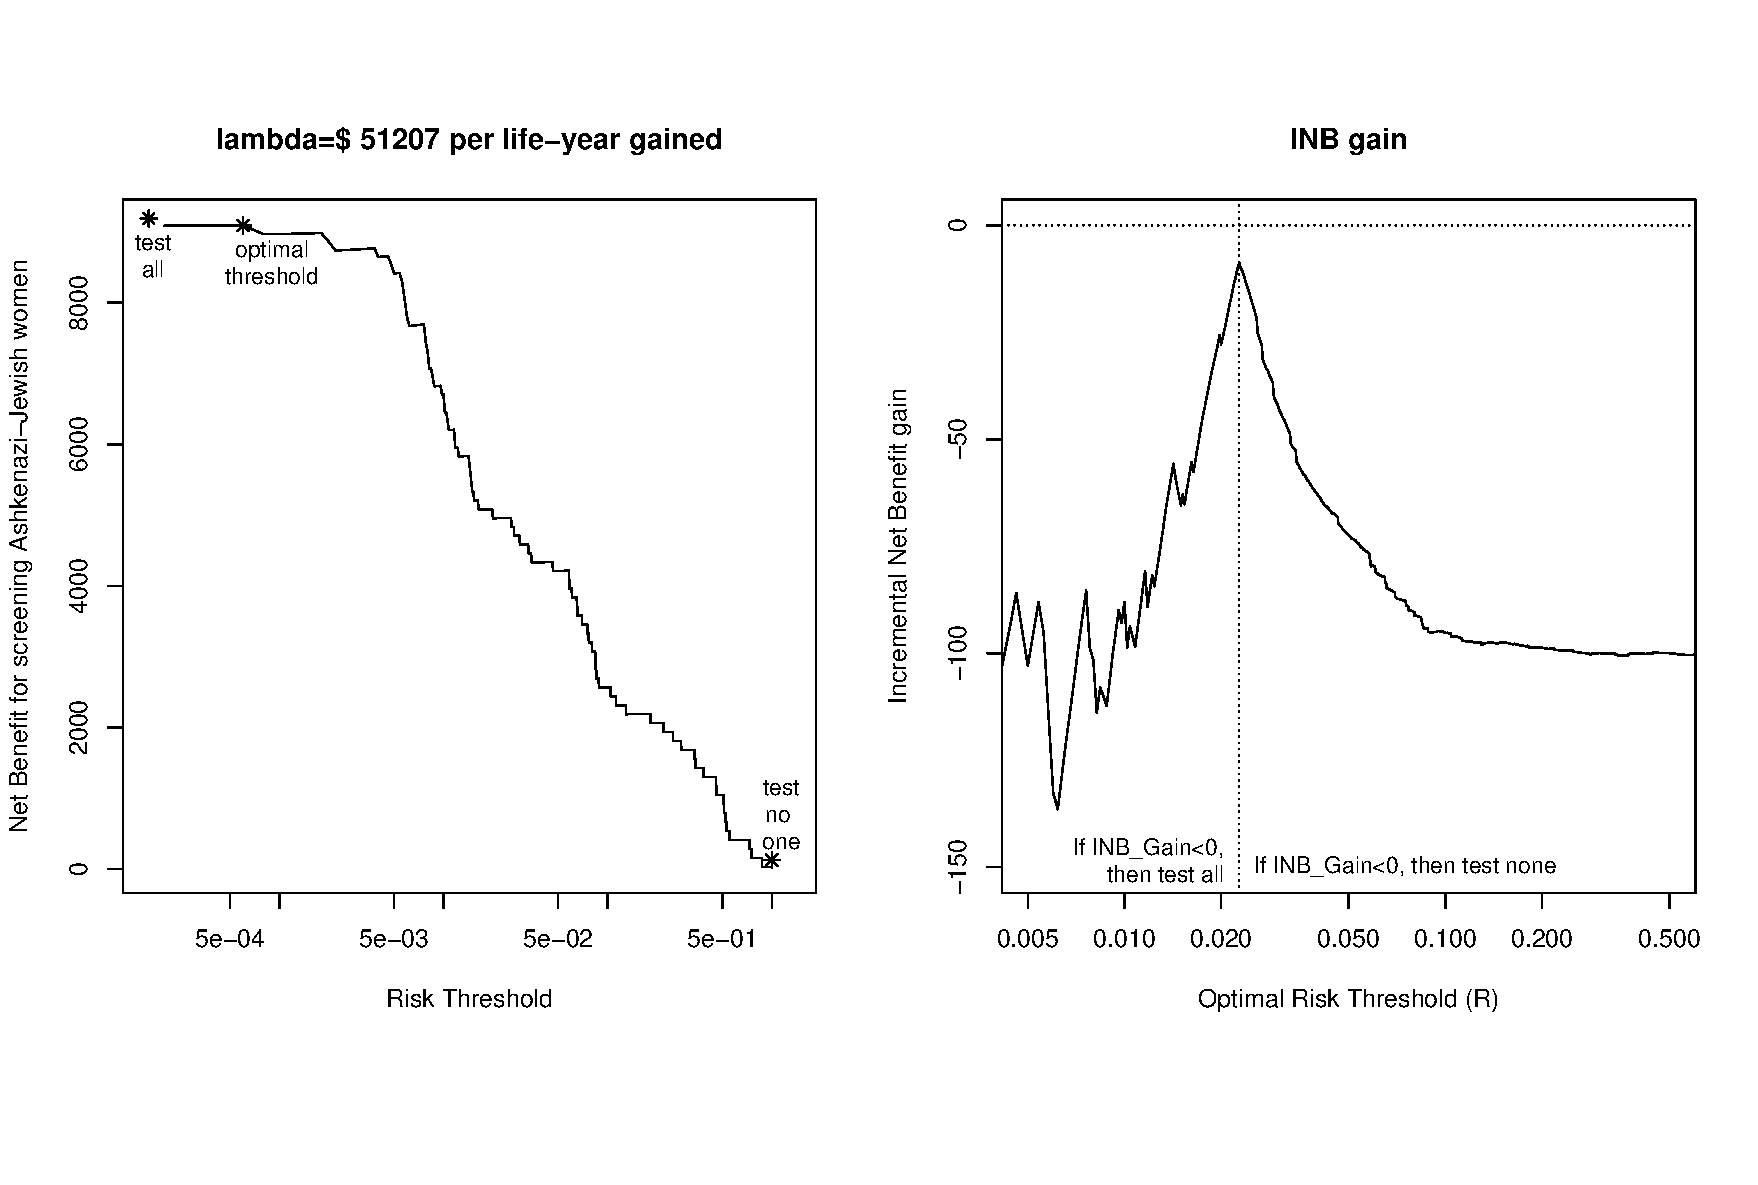
\includegraphics[angle=-0,width=5.5in,]{Fig1AJ.pdf}
	\caption{Left panel is Net Benefit for screening vs. risk threshold for using the BRCAPRO risk model to screen for which Ashkenazi-Jewish women should get \textit{BRCA1/2} genetic testing.  The optimal risk threshold is marked, as are the Net Benefits for testing no one or testing everyone.  The right panel plots $I\!N\!B_{Gain}(R)$ vs. optimal risk threshold.  The vertical line is where the optimal risk threshold equals disease prevalence.  To the left of the vertical line, if the INB gain is negative, then the testing everyone is the preferred policy.  To the right of the dotted line, if the INB gain is negative, then the testing no one is the preferred policy.  For optimal risk thresholds where INB gain is positive, screening is the preferred policy.}
	\label{fig:1AJ}
\end{figure}

Figure~\ref{fig:1AJ} (left panel)  shows that the Net Benefit of using BRCAPRO increases as the risk threshold decreases.  For a willingness to pay of $\lambda=\$51,207$ per life-year gained, the optimal risk threshold is $c_0/(e(\lambda)+c_0) = 249/(414751+249)=0.06\%$.  However, testing all has the highest Net Benefit, and thus would be the preferred policy for $\lambda=\$51,207$.  The only part of the curve of Figure~\ref{fig:1AJ} (left panel) that matters is the Net Benefit at the optimal risk threshold, because other thresholds are suboptimal for $\lambda=\$51,207$.  Thus, for each $\lambda$, we calculate its associated optimal threshold (equation~\ref{eq:dollarsperLYG}) and the Net Benefit only at the optimal threshold.  We compare the optimal Net Benefit for screening at each optimal threshold versus the Net Benefits for testing no one or testing everyone  (Figure~\ref{tab:NBforAJ}).  A key point is that as threshold $R$ decreases, its associated willingness to pay $\lambda$ increases.  Although each threshold in the table is optimal for a given willingness to pay, many of these $\lambda$ will be infeasible for anyone.  For example, at the 0.02\% threshold, the $\lambda=\$217,206$ is outside the typical range of willingness to play (\$10,000 to \$100,000), and is probably not feasible for anyone.  Furthermore, note that thresholds above 0.16\% imply \textit{negative} willingness to pay, meaning that life-gained is devalued.  These thresholds are immoral and cannot be considered.  Thus the only optimal thresholds that can be considered are 0.04\% to 0.12\%.

\begin{figure}[t!]
	\centering
	\begin{verbatim}
  Threshold   lambda  NB_M(R)  NB_none   NB_all INB_gain(R)
     0.0002 217206.7 17365663 17337699 17365763   -99.54
     0.0004  92706.7  7411327  7397518  7411425   -98.55
     0.0006  51206.7  4093217  4084124  4093313   -96.10
     0.0008  30456.7  2434068  2427427  2434257  -188.92
     0.0010  18006.7  1438656  1433409  1438823  -166.80
     0.0012   9706.7   775049   770730   775200  -151.37
     0.0014   3778.1   301046   297389   301184  -138.67
     0.0016   -668.3   -54456   -57618   -54328  -128.54
     0.0018  -4126.6  -330957  -333734  -330837  -119.40
	\end{verbatim}
	\caption{Optimal thresholds, their associated willingness to pay $\lambda$, and the Net Benefits of screening $N\!B_M(R)$,  testing no one $N\!B_{none}$, and testing everyone $N\!B_{all}$, and the INB gain of screening versus the better of testing no one or testing everyone $I\!N\!B_{Gain}(R)$.}
	\label{tab:NBforAJ}
\end{figure}

The Net Benefit for screening at the optimal threshold $N\!B_M(R)$ increases as threshold $R$ decreases.  However, the $I\!N\!B_{Gain}$ is negative, meaning that either testing no one or testing everyone is the best policy versus each optimal threshold.  Specifically, the Net Benefit for testing everyone $N\!B_{all}$ is highest at each optimal threshold and is thus the best policy.  Figure~\ref{fig:1AJ} (right panel) plots the $I\!N\!B_{Gain}(R)$.  See Figure~1 of the WebAppendix to see $I\!N\!B_{none}$ and $I\!N\!B_{all}$ separately 

The $I\!N\!B_{Gain}(R)$ always peaks at $R=P(D+)$ disease prevalence, and thresholds where $I\!N\!B_{Gain}(R)>0$ favor screening as the policy.  Since $I\!N\!B_{Gain}(R)$ is negative at all optimal risk thresholds, then either testing no one or testing all are the preferred policies, depending on what the feasible optimal risk thresholds are.  Since only thresholds from 0.04\% to 0.12\% are feasible, then the preferred policy is testing everyone.



\subsection{Effect of ignoring screening test cost}
\label{sec:IgnoreScreeningTestCost}

\begin{figure}[t!]
	\centering
	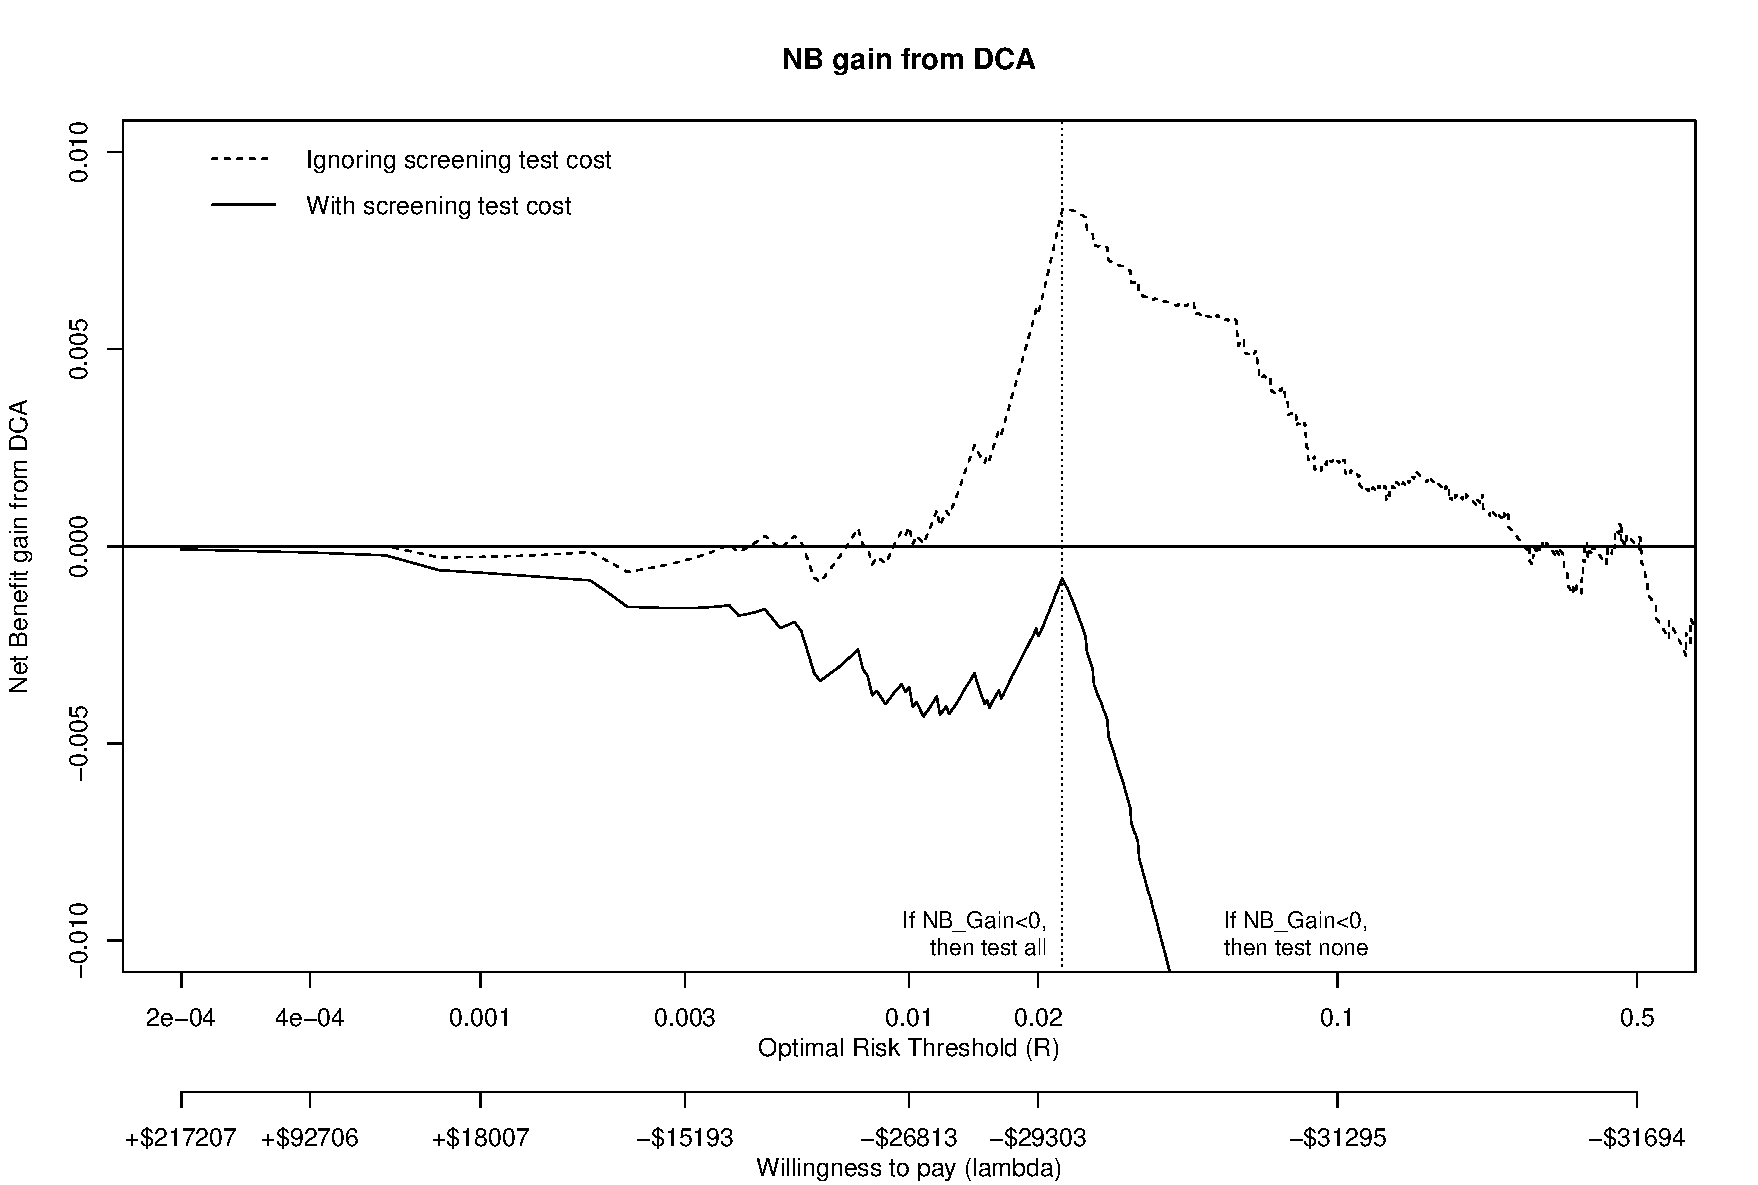
\includegraphics[angle=-0,width=5.5in,]{testcostsAJ.pdf}
	\caption{NB gain from Decision Curve Analysis (DCA) (both ignoring and with screening test cost) vs. BRCAPRO risk-threshold to screen for which Ashkenazi-Jews should get \textit{BRCA1/2} genetic testing.  The second x-axis plots the associated willingness to pay $\lambda$ for each optimal risk threshold $R$. The vertical line is where the optimal risk threshold equals disease prevalence.  To left of this line, if $N\!B_{Gain}$ is negative then testing everyone is the favored policy; to the right, testing no one is favored.}
%	\caption{NB gain from Decision Curve Analysis (DCA) (left panel) vs. BRCAPRO risk-threshold to screen for which Ashkenazi-Jews should get \textit{BRCA1/2} genetic testing.  The right panel plots NB gain from DCA for a costless BRCAPRO screening test versus the dollars per life-year gained implied by each optimal risk-threshold.  The vertical line is where the optimal risk threshold equals disease prevalence.  To left of this line, if NB gain is negative then testing everyone is the favored policy; to the right, testing no one is favored (vice versa for the right plot).}
	\label{fig:testcostsAJ}
\end{figure}

Figure~\ref{fig:testcostsAJ} shows that the NB gain from Decision Curve Analysis (DCA), with BRCAPRO screening test cost $c_m=\$100$ (middle panel), is always negative.  Thus screening is never the best choice.  However, the NB gain estimated by usual costless test assumption shows that screening is the best choice for a wide range of risk thresholds from 1\% to 30\%.  Thus \textit{BRCA1/2} mutation screening is sensitive to a small BRCAPRO screening test cost.  It is hard to see this sensitivity from the costless NB gain because its units are abstract.  In contrast, this sensitivity is easy to see from INB gain (Figure~\ref{fig:1AJ}, right panel) because its units are dollars.  The INB asymptotes at -\$100, clarifying that a \$100 cheaper screening test would permit screening at a wide range of risk-thresholds.

Figure~\ref{fig:testcostsAJ} (right panel) plots NB (for a costless BRCAPRO test) versus the threshold for dollars per life-year gained, using equation~\ref{eq:dollarsperLYG} to convert from optimal risk threshold to dollars per life-year gained.   The wide range of risk thresholds supporting screening for a costless BRCAPRO test implies that the threshold for dollars per life-year gained is \textit{negative}.  This means that doing genetic testing on all Ashkenazi-Jewish women is not merely cost-effective, but is actually \textit{cost-saving}, versus screening with BRCAPRO at optimal thresholds.  The reason for the negative dollars per life-year gained is that the difference in treatment costs for early- vs. late-detection $c_1-c_2=-\$158717$ is strongly negative.  Thus our framework clarifies that the reason why testing all Ashkenazi Jews saves money versus screening with BRCAPRO is because treating cancer is far more expensive than treatment costs incurred by genetic testing.

This example demonstrates that optimal risk thresholds can imply infeasible thresholds of dollars per life-year gained.  Note that dollars per life-year gained thresholds cannot be calculated by DCA and requires specifying costs and effectiveness.

Our conclusion agrees with that of microsimulation-based decision analyses that more comprehensively considered costs and effectiveness, but only examined screening at a single implicit risk-threshold~\citep{Long2015,Manchanda2015}.  The usefulness of our simple framework is that we examine all risk thresholds easily and it is easy to understand why a conclusion is reached.  



%This is not overcome by the cost increase due to genetic testing because $c_0$ is only $\$249$, the smallest optimal threshold is $R\approx1\%$, and thus $c_0(1-R)/R\approx\$25000$ . 



\subsection{\textit{BRCA1/2} mutation screening for the general population}
\label{sec:BRCAgenpop}

\begin{figure}[t!]
	\centering
	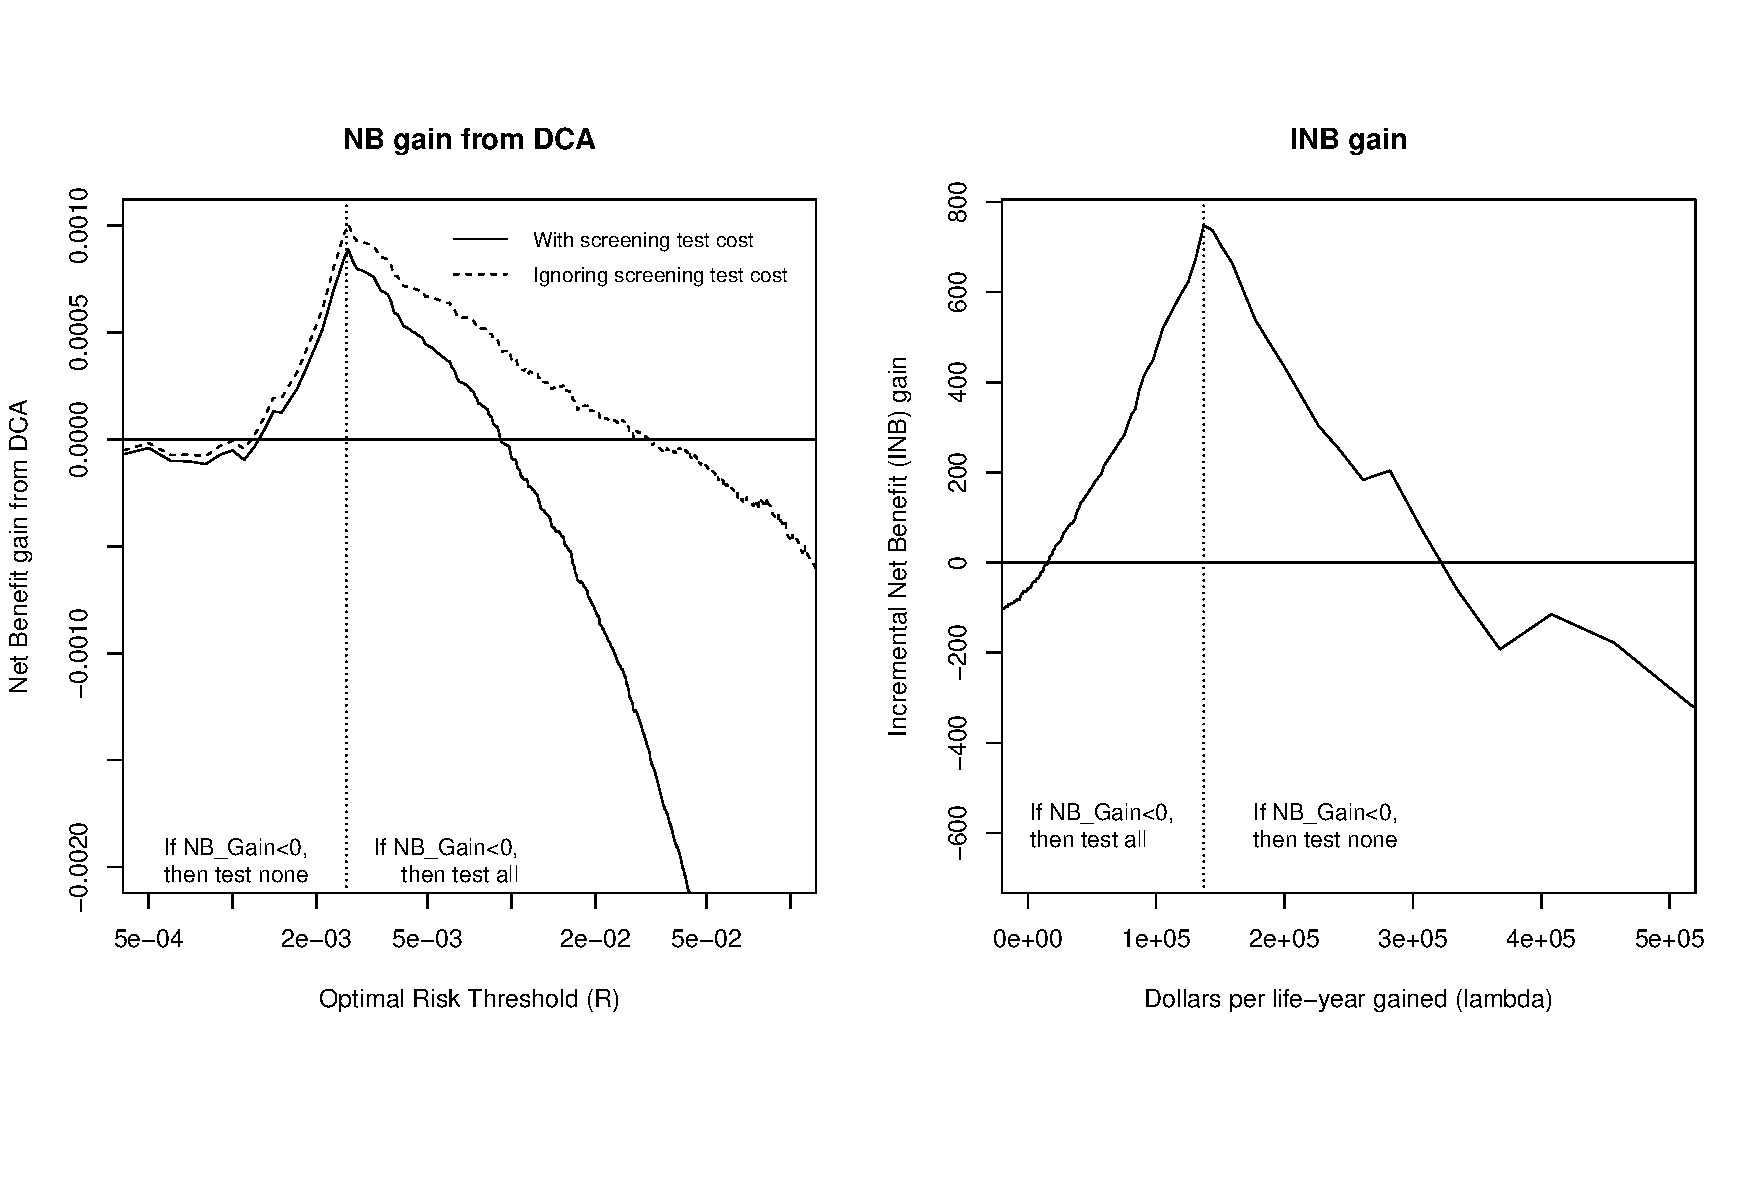
\includegraphics[angle=-0,width=6.5in,]{testcostsGenPop.pdf}
	\caption{NB gain from Decision Curve Analysis (DCA) vs. risk-threshold (left panel) and INB gain vs. dollars per life-year gained (right panel) for using the BRCAPRO risk model to screen for which members of the general population should get \textit{BRCA1/2} genetic testing.}
	\label{fig:testcostsGenPop}
\end{figure}

In the general population, \textit{BRCA1/2} mutations have only 0.26\% prevalence (10 times lower than in Ashkenazi-Jews).  

Figure~\ref{fig:testcostsGenPop} (left panel) shows that accounting for just a \$100 screening BRCAPRO test cost greatly reduces the range of allowable risk thresholds for screening, from $(0.12\%,3.1\%)$ to $(0.13\%,0.91\%)$.  Figure~\ref{fig:testcostsGenPop} (right panel) shows that screening with BRCAPRO is cost-effective at dollars per life-years gained thresholds ranging from $(\$16,\!000,\$306,\!000)$, which spans typical thresholds for Western countries.  The peak INB of \$700 shows that a BRCAPRO screening that cost \$700 more (total $c_m=\$800$) would be required for screening to never be the preferred policy, which is unreasonably expensive for shared decision-making.  

The dollars per life-year gained at peak INB is $\$137,\!000$, which is high even for the US.  Figure~\ref{tab:dollarsperLYG} shows the performance of screening along the range of allowable thresholds of dollars per life-year gained.  As dollars per life-year gained increases, so does the fraction of mutation carriers identified (sensitivity; from 40\% to 67\%) but also the fraction of women referred for genetic testing (6.4\% to 28\%).  Note that sensitivities below 40\% do not support screening (instead screen none: sensitivity is 0\%) and neither do sensitivities above 67\% (instead test everyone; sensitivity is 100\%) The predictiveness of BRCAPRO increases from AUC of 0.669 to 0.698 at peak INB, then levels off.  

The more comprehensive analysis of Long and Ganz~\cite{Long2015} suggests that testing everyone is cost-effective at \$920,000 per QALY.  Most of this increase is due to quality adjustment, which roughly halved the value of life-years gained.  If we halve the life-years gained due to screening (to 2.5), then testing everyone is cost-effective at \$612,000 per life-year gained, much closer to Long and Ganz~\cite{Long2015}.  Our approach reaches the same practical conclusion as the comprehensive decision-analysis, while also considering different risk thresholds.  Our approach as allows for simple understanding of why cost-effectiveness is reduced in the general population versus in Ashkenazi-Jews:  the cost of definitive genetic testing $c_0$ is much higher, and the mutations are 10 times rarer.

\begin{figure}[t!]
	\centering
	\begin{verbatim}
 Dollars/LYG Threshold INBgain Positivity      PPV     cNPV   Sens   Spec    AUC
       20197    0.0084   27.74    0.06377 0.016048 0.001640 0.4000 0.9371 0.6685
       50835    0.0053  171.90    0.09364 0.012295 0.001553 0.4500 0.9073 0.6786
      101150    0.0033  482.62    0.12929 0.010059 0.001445 0.5083 0.8717 0.6900
      137047    0.0026  748.35    0.14741 0.009401 0.001375 0.5417 0.8536 0.6976
      199395    0.0019  436.65    0.18377 0.008006 0.001332 0.5750 0.8172 0.6961
      306278    0.0013   76.46    0.28016 0.006164 0.001155 0.6750 0.7209 0.6979
	\end{verbatim}
	\caption{Peformance of using BRCAPRO to screen for \textit{BRCA1/2} mutations at various dollars per life-year gained thresholds that favor screening in the general population.}
\label{tab:dollarsperLYG}
\end{figure}


%\section{Simple condition for a screening test to have greater INB}
%\label{sec:moreINB}
%
%%If one screening test has greater sensitivity and greater specificity than another, then it is obvious that first test is better without any cost-effectivenss analysis.  However, 
%
%IONUT:  I DON'T THINK THIS FITS IN HERE.  I THINK IT SHOULD BE ITS OWN PAPER.
%
%Usually one screening test has better sensitivity but another has better specificity.  Informational metrics like Youden's index, MRS, AUC, and NB do not explicitly consider costs and effectiveness and are all optimized when risk threshold equals disease prevalence.  Ideally, the sensitivity vs. specificity tradeoff would be evaluated considering costs and effectiveness via the INB.
%
%For two markers $M_1$ and $M_2$ with equal marker cost, then $\Delta INB=INB_1-INB_2>0$ if
%\begin{eqnarray*}
%	\Delta INB &=& (e+c_0)[P(D+,M_1+)-P(D+,M_2+)] - c_0[P(M_1+)-P(M_2+)]\\
%	&=& (e+c_0)[Sens_1-Sens_2]\pi - c_0[p_1-p_2] > 0
%\end{eqnarray*}
%for disease prevalence $P(D+)=\pi$, sensitivities $Sens_i=P(M_i\!+|D+)$, and test-positivities $P(M_i+)=p_i$.  Choosing test 1 so that $Sens_1>Sens_2$, then presuming $p_1>p_2$,
%\begin{eqnarray}
%\label{eq:SensMoreINB}
%	\frac{Sens_1-Sens_2}{p_1-p_2} &>& \frac{c_0/[e+c_0]}{\pi} = \frac{R}{\pi}.
%\end{eqnarray}
%The simple condition examines if the slope of the concentration curve is less than a constant.  This constant is the ratio of the optimal risk threshold $R$ to the disease prevalence, which is the optimal threshold under information metrics such as Youden's index, AUC, MRS, and Net Benefit, none of which specify costs and effectiveness.  Thus the key is the ratio of optimal risk thresholds by considering costs and effectiveness versus ignoring them.  If $R=\pi$, then increases in sensitivity and test-positivity are weighed equally.  If $R<\pi$ which means we should be testing more people, then we will accept smaller sensitivity gain for a larger test-positivity increase.  But if $R>\pi$, meaning we should be testing fewer people, then we require a greater sensitivity gain than a test-positivity increase.  The WebAppendix shows an equivalent condition based on specificity. 
%
%Note that if $p_1<p_2$, then the inequality flips and the left side is negative while the right is positive: test 1 is always better if it has higher sensitivity yet lower test-positivity (equivalent to higher sensitivity and higher specificity), as long as the two screening test costs are equal.   However, if the two screening test costs are unequal, $\Delta INB=INB_1-INB_2>0$ if
%%\begin{eqnarray*}
%%	\Delta INB &=& (e+c_0)[P(D+,M_1+)-P(D+,M_2+)] - c_0[P(M_1+)-P(M_2+)] - [c_{m1}-c_{m2}]\\
%%	&=& (e+c_0)[Sens_1-Sens_2]\pi > c_0[p_1-p_2] + [c_{m1}-c_{m2}]\\
%%	&=& [Sens_1-Sens_2]\pi/\pi_{INB} > [p_1-p_2] + [c_{m1}-c_{m2}]/c_0
%%\end{eqnarray*}
%%for disease prevalence $P(D+)=\pi$ and test-positivities $p_1,p_2$.  The required condition is
%\begin{eqnarray}
%\label{eq:MoreINBunequalCosts}
%	[Sens_1-Sens_2]  &>& \frac{R}{\pi} \left( [p_1-p_2] + \frac{c_{m1}-c_{m2}}{c_0} \right),
%\end{eqnarray}
%where $c_{mi}$ is the cost of screening test $i$.  Compared to equation~\ref{eq:SensMoreINB}, this equation also includes the ratio of the increase in screening test cost to the definitive test cost.  Unlike for equal test costs, if screening test 1 has both better sensitivity and smaller test positivity, but a big increase in screening test cost compared to definite test cost, then test 1 may be too expensive to be cost-effective.  
%
%\subsection{Examples}
%\label{sec:90vs80}
%
%\cite{Best2019} showed a concentration curve for the fraction of \textit{BRCA1/2} mutation carriers identified (sensitivity) versus the fraction of women who test positive by BRCAPRO.  They focus on two thresholds: a "Test 1" that identifies 90\% of mutation carriers by testing 60\% of women, and a "Test 2" that identifies 80\% of mutation carriers by testing 44\% of women.  The AUC for Test 1 vs. Test 2 is 0.658 vs 0.688, respectively.  We examine which threshold is more cost-effective.  
%
%(IONUT:  the weakness of these examples is that 80\% or 90\% sensitivity is never preferred versus testing everyone.  Maybe I need to modify).
%
%Since these are two thresholds for the same test (BRCAPRO), the test costs are by definition equal.  Given the effectiveness and cost for screening 50-year old women (section~\ref{sec:CostsEffBRCA}) and setting dollars per life-year gained at $d=\$50,\!000$, then $e=\$408,\!717$ (we fix this throughout this section).  Thus $R=2200/(408717+2200)=0.54\%$.  Since \textit{BRCA1/2} mutation prevalence is $\pi=0.26\%$, the critical slope is $R/\pi=2.1$.  The slope of the concentration curve is $(0.9-0.8)/(0.6-0.44)=0.625$.  Since the slope is less than the critical slope, condition~\ref{eq:SensMoreINB} is not satisified, and thus Test 2 is more cost-effective.  By equation~\ref{eq:SensMoreINB} the minimum dollars per life-year gained is $d=\$243,\!000$ for test 1 to be more cost-effective than test 2.
%
%%\cite{Best2019} report that, if extra time is taken to elicit cancer family history on aunts, cousins, and more distant relatives, then 80\% of mutation carriers were identified by testing only 35\% of women.  This test is statistically superior to Test 2 because it tests fewer women than Test 2 yet identifies the same fraction of mutation carriers.  However, eliciting more family history takes more time, and perhaps shared decision-making costs \$100 more ($c_{m1}=\$200$ vs. $c_{m2}=\$100$).  The condition~\ref{eq:MoreINBunequalCosts} is not satisfied because the sensitivity gain is 0, but the right side is -0.09.  Thus the superior statistical performance of eliciting additional family history is also cost-effective.  
%
%\cite{Best2019} also provide a simple modification to National Comprehensive Cancer Network (NCCN) guidelines so that 90\% of mutation carriers are identified by testing 68\% of women.  These simple guidelines are statistically inferior to the BRCAPRO threshold at which 90\% of carriers are identified by testing only 60\% of women.  However, since these simple guidelines do not require a BRCAPRO risk calculation, perhaps the screening test is \$50 cheaper ($c_{m1}=\$50$ vs. $c_{m2}=\$100$).  The condition~\ref{eq:MoreINBunequalCosts} is not satisfied because the sensitivity gain is 0, but the right side is 0.12.  Thus screening with the simple modification to NCCN guidelines is not cheap enough to be cost-effective versus screening with BRCAPRO.  Even if the NCCN modification were costless, by equation~\ref{eq:MoreINBunequalCosts}, it would still not be more cost-effective than screening with BRCAPRO.



% OLD STUFF
%As a hypothetical example, assume a new screening test can identify 90\% of mutation carriers by testing only 40\% of women.  It is statistically superior to Test 2 because it tests fewer women than Test 2 yet identifies more mutation carriers.  However, the new test costs \$150 more ($c_{m1}=\$250$ vs. $c_{m2}=\$100$).  The condition~\ref{eq:MoreINBunequalCosts} is not satisfied because the sensitivity gain is 0.10, but the right side is 0.17.  Thus the new test may have superior statistical performance, but its higher cost renders it less cost-effective.  The new test would have to cost no more than $c_{m1}=\$204$ for it to be more cost-effective than Test 2.

%Note that these inequalities do not require that two markers be dichotmized at the optimal threshold $R$, or even at the same threshold.  For example, the Pap and HPV tests are implicitly categorized at different thresholds, neither of which is necessarily optimal.  However, this leaves open the question that the comparison is unfair, much less suboptimal.  If the two markers are dichotomized at the same risk-threshold, it's a most fair comparison, and if the risk threshold is also $\pi_{INB}$, then the comparison is definitive.


% The equivalent condition in terms of MRS is:
% \begin{eqnarray*}
% \Delta INB &=& [MRS_1-MRS_2](e+c_0)/2 - [p_1-p_2][c_0-\pi(e+c_0)] >0
% \end{eqnarray*}
% or 
% \begin{eqnarray*}
% \frac{MRS_1-MRS_2}{p_1-p_2} &>& 2\frac{c_0-\pi(e+c_0)}{e+c_0} = 2(\pi_{INB}-\pi).
% \end{eqnarray*}
% Note that this presumes that $p_1>p_2$, reverse the inequality otherwise.  It's interesting that the condition depends on the difference of optimal INB risk threshold versus optimal MRS threshold.  This means that, if $p_1>p_2$, marker 1 can have worse MRS yet better INB, but the optimal INB threshold must be less than prevalence (meaning, you should be testing more people anyway), and the MRS is not too much worse.  Thus, a marker 1 with worse MRS for $p_1>p_2$ for $\pi_{INB}>\pi$, where you should be testing fewer people, can never be better.  The equivalent expression via Youden's index J (via $MRS=2J\pi(1-\pi$)) is
% \begin{eqnarray*}
% \frac{J_1-J_2}{p_1-p_2} &>& \frac{\pi_{INB}-\pi}{\pi(1-\pi)}.
% \end{eqnarray*}
% This is all interesting, but complex to explain, and provides no extra insight versus the conditions based on sensitivity and specificity.



% \section{Minimum MRS needed for a biomarker to be better than testing no one or testing everyone}
% 
% How much MRS do we need to ensure that using the marker is better than testing no one or testing everyone?  This would set the minimum MRS necessary, and give scientists an objective MRS goal to shoot for when designing new biomarker tests.  Let's presume $MRS>0$ and $e>0$, else we never screen.  
% 
% I've commented out some work below because I need to think about it more, and I just want to send you what I have right now.




\section{Sensitivity Analyses}
\label{sec:SensAnaly}

An important part of any decision analysis is assessing sensitivity to the input parameters.  As noted in section~\ref{sec:BRCAAJs}, the INB is on the scale of the screening test cost $c_m$, so visually inspecting a plot like figure~\ref{fig:testcostsGenPop} (right panel) makes it easy to assess sensitivity to screening test cost.  Below we consider sensitivity to other parameters.

\subsection{Different effectiveness and treatment costs affects dollars per life-year gained, but not optimal risk thresholds}
\label{sec:40vs50}

The optimal risk threshold $R=c_0/(e+c_0)$ is a function of only definitive test cost $c_0$ and net effectiveness $e=\lambda(e_1-e_2)-(c_1-c_2)$.   Thus, if $R$ is fixed (as in DCA or plots of INB gain vs $R$), then also fixing $c_0$ means that $e$ is determined.  Thus if the life-years gained $(e_1-e_2)$ or gain in treatment costs $(c_1-c_2)$ changes, then the willingness to pay $\lambda$ will adapt to ensure that $e$ remains fixed.  Thus optimal risk thresholds are entirely unaffected by changing the effectiveness or treatment costs, because $\lambda$ varies to ensure that $e(\lambda)$, and hence $R$, remain fixed.  However, the meaning of the risk threshold in terms of dollars per life-year gained will be altered.  The associated dollars per life-year gained thresholds are readily calculated by plugging quantities into equation~\ref{eq:dollarsperLYG}.

For example, if the life-years gained $(e_1-e_2)$ increases to 6.5 from 5.0, the plot of INB gain or NB gain from DCA, versus risk threshold, such as figure~\ref{fig:testcostsGenPop}, is unaltered (not shown).  The risk-thresholds for which BRCAPRO screening is viable in the general population remains $(0.13\%,0.91\%)$ in spite of the increase in effectiveness.   However, because life-years gained increased, equation~\ref{eq:dollarsperLYG} calculates that the dollars per life-year gained threshold implied by these thresholds now decreases to $(\$12,\!000,\$240,\!000)$.   Similarly, if the difference in treatment costs $(c_1-c_2)$ is halved, the risk-thresholds supporting screening remain $(0.13\%,0.91\%)$, but their associated dollars per life-year gained thresholds now increase to $(\$32,\!000,\$322,\!000)$ because screening saves less money.

%By equation~\ref{eq:INBgain}, INB is a function of only risk threshold $R$, definitive cost $c_0$, and screening marker cost $c_m$.  Thus fixing $R=c_0/(e+c_0)$ (and $c_0$ and $c_m$) yields the same INB and fixes the value of net effectiveness $e=d(e_1-e_2)-(c_1-c_2)$.  


\subsection{Sensitivity to cost of the definitive test}
\label{sec:SensitivityC0}

In contrast, by equation~\ref{eq:INB_Gain}, varying $c_0$ (fixing $R$ and $c_m$) changes the toptimal risk thresholds $R$.  This can be examined empirically by plugging in different $c_0$.  For example, if the cost of \textit{BRCA1/2} genetic testing in the general population was halved from \$2200 to \$1100, the range of risk thresholds supporting screening shrinks from $(0.13\%,0.91\%)$ to $(0.14\%,0.68\%)$ and their associated dollars per life-year gained thresholds improve from $(\$16,\!000,\$306,\!000)$ to $(\$3,\!000,\$125,\!000)$.

A pressing sensitivity analysis is the critical cost of definitive \textit{BRCA1/2} genetic testing at which testing all women in the general population is better than any screening.  This can be found by solving for $c_0$ in $I\!N\!B_{Gain}=0$, while fixing dollars per life-year gained (i.e. fixing net effectiveness $e$):
\begin{eqnarray*}
	c_0 &=& \frac{c_m+e(\lambda)\cdot P(D+,M-)} {P(D-,M-)}.
\end{eqnarray*}
The critical cost, calculating $e(\lambda)$ by fixing the dollars per life-year gained threshold at $\lambda=\$0$, represents a minimal cost at which genetic testing for all women is the best decision, because $\lambda$ is the lowest ethical willingness to pay.  For $\lambda=0$, the critical cost of \textit{BRCA1/2} genetic testing is \$397.  Thus, if the cost of \textit{BRCA1/2} genetic testing in the general population fell to \$397, then testing all women is preferred versus screening, regardless of your threshold for dollars per life-year gained.  Of course, any real willingness to pay threshold will be higher than 0, allowing higher critical definitive test costs.  At willingness to pay thresholds of \$20,000, \$50,000, and \$100,000, the critical costs of \textit{BRCA1/2} genetic testing are \$532, \$746, and \$1068, respectively.  Although \$1000 \textit{BRCA1/2} testing will be achieved soon, \$400 testing may take some time to achieve.





%\subsection{With respect to input parameters}
%
%It is common in cost-effectiveness to see how sensitive the results are (i.e., INB herein) with respect to changes in input parameters. The input parameters are the cost (i.e., $c_0$, $c_1$, $c_2$ and $c_m$)and the effectiveness (i.e., $e_1$ and $e_2$) parameters. Since INB is linear in these parameters and $P(D+,M+)$ and $P(M+)$ are assumed fixed, it is straightforward to assess the sensitivity of the results (e.g., assuming these cost and effectiveness input parameters are normally distributed yields a normally distributed INB).  HK: NOT QUITE.  $P(D+,M+)$ and $P(M+)$ ARE IMPLICITLY FUNCTIONS OF THE OPTIMAL CUTPOINT FOR M OF $c_0/(e+c_0)$ AND THUS THE INB IS NON-LINEAR IN ALL PARAMETERS EXCEPT $c_m$.
%
%\subsection{With respect to the risk-model}
%
%\textcolor{blue}{\it Now that I look at it in this way, the model in Section 3 could be thought of as allowing for error in the risk-model (still unbiased, but with some random error), hence it is a sensitivity analysis. Could you please provide density plots for the risk marker $M$ in AJ and the general population? Separately, we want to see whether we could employ some parametric model.}
%
%IONUT: LET'S NOT BOTHER WITH THIS, LET'S SAVE THIS FOR FUTURE WORK.

% \subsection{INB for testing no one or testing everyone}
% 
% Note $pi_{INB}$ finds the interior maximum for $INB(m_0)$.  The boundaries of testing no one and testing everyone have to be compared to $INB(\pi_{INB})$ to see which is greatest. If we test no one, then $INB=0$.  If we test everyone, we can set $c_m=0$ since we don't need the marker, and
% \begin{eqnarray*}
%   INB_{all} &=& [(e_1-e_2)-(c_1-c_2-c_0)]\pi - c_0\\
%             &=& [e+c_0]\pi - c_0, 
% \end{eqnarray*}
% and thus we have an intuitive form for INB:
% \begin{eqnarray*}
%   INB &=& (e+c_0)MRS/2 - c_m + p[e\pi + c_0\pi - c_0] \\
%       &=& (e+c_0)MRS/2 - c_m + pINB_{all}.
% \end{eqnarray*}
% 
% \subsection{Minimum MRS, and maximum marker cost, for using marker to beat testing no one}
% 
% For beating testing no one (INB=0), set the INB equation above to be greater than zero and solve for MRS:
% \begin{eqnarray*}
%   MRS &>& 2\frac{c_m-pINB_{all}}{e+c_0}
% \end{eqnarray*}
% The right side is maximized if $p=0$.  Thus the minimum MRS for the biomarker to beat testing no one is
% \begin{eqnarray*}
%   MRS_{min} &=& 2\frac{c_m}{e+c_0}.
% \end{eqnarray*}
% Marker cost is key for setting this minimum MRS, which only depends on utilities.  Recall that the maximum MRS for a disease is $2\pi(1-\pi)$.  This also sets a maximum marker cost, beyond which it is not cost-effective to use even a perfect test:
% \begin{eqnarray*}
%   c_m &\le& \pi(1-\pi)(e+c_0)
% \end{eqnarray*}
% 
% \subsection{Minimum MRS, and maximum marker cost, for using marker to beat testing everyone}
% 
% For beating testing everyone ($INB=INB_{all}$), set the INB equation above to be greater than $INB_{all}$ and solve for MRS:
% \begin{eqnarray*}
%   MRS &>& 2\frac{c_m+(1-p)INB_{all}}{e+c_0}
% \end{eqnarray*}
% For the biomarker to beat testing everyone,



\section{Discussion}
\label{Discussion}

We proposed a simple framework for identifying optimal risk-thresholds for a single-time screening test.  Our framework provides a simple equation not only for the optimal risk-threshold, but more importantly, also for the dollars per life-year gained underlying an optimal risk-threshold.  The dollars per life-year gained threshold is necessary to know which optimal risk-thresholds are feasible in practice.  Because the dollars per life-year gained is a value that differs between people and societies, we plot the gain in Incremental Net Benefit (INB) versus the dollars per life-year gained threshold to identify the optimal risk-thresholds that support screening.  Because the INB is on the scale of screening test cost, it easily identifies sensitivity to screening test costs.  Although optimal thresholds are invariant to effectiveness and treatment costs, the dollars per life-year gained associated with the threshold can change substantially with effectiveness and treatment costs.  Our framework relies only on simple closed-form expressions that are easy to query for sensitivity to costs and effectiveness to better understand the conclusions drawn by the INB.

Our framework fills a niche as a bridge between Decision Curve Analysis (DCA) and a full-blown proper decision-analysis.   DCA is the natural next step following an analysis of statistical properties such as classification ability and risk stratification, as it introduces the decision-analytic concept of optimal risk-thresholds without requiring specification of costs or effectiveness~\citep{Katki2019}.  However, because costs and effectiveness are not specified, DCA cannot identify optimal risk-thresholds.  In practice, DCA is usually conducted with a costless screening test assumption.  This assumption may seem reasonable when the screening test is a risk model, but risk models usually require shared decision-making in practice.  We showed that, DCA can account for screening test costs, but at the cost of requiring that all costs and effectiveness also be specified, which negates the simplicity of use of DCA in practice.  Because, DCA is on the abstract scale of Net Benefit, it can be difficult to see whether the DCA is sensitive to screening test cost.  Most importantly, while DCA can identify a range of thresholds that support screening, it cannot assess their associated dollars per life-year gained, which is necessary to know which thresholds are feasible.  Our framework could be the next step after DCA to quickly and easily examine the importance of different quantities and structural assumptions, to help plan the final and comprehensive decision-analysis.

In contrast, a full decision-analysis requires specifying not only costs and effectiveness, but also all possible decisions for different people.  This approach is the most comprehesive "final" answer for identifying optimal risk thresholds.  However, comprehensive decision-analyses usually require complex methods, such as decision-trees or microsimulation.  These methods, although powerful and comprehensive, can be hard to understand why they arrive at their conclusion.  Probabilistic sensitivity analysis helps, but readers of such papers usually do not have access to the computational model to personally assess sensitivity to inputs and structural assumptions.  We suggest that comparing answers from our approach to a comprehensive approach can help informs each other.  If the two approaches agree, then either complexities don't matter or they happen to cancel each other's effects.  If don't agree, either the our approach is missing something critical or the comprehensive approach may be speculatively modeling something incorrectly.  Resolving the disagreement could prove insightful and advance the debate on what is cost-effective, and spur reseach into any quantities identified as being critical but poorly known.

In the \textit{BRCA1/2} example, DCA, under the usual costless screening test assumption, identified a wide range of risk thresholds (1\%-30\%) supporting screening among Ashkenazi-Jews.  But allowing a mere \$100 cost for shared decision-making wiped out all the thresholds and made clear the best decision is to do genetic testing for all Ashkenazi-Jewish women.  The DCA uses the abstract scale of Net Benefit, so it is hard to see this sensitivity, but easy via the INB which is on the scale of the cost of the screening test.  In the general population, risk thresholds from (0.13\%-0.91\%) support screening.  However, not all of these will be feasible in practice because they represent dollars per life-year gained thresholds from $\$16000-\$306000$; typical thresholds in practice are below \$100,000.   This example shows that knowing the optimal thresholds does not suffice; the dollars per life-year gained associated with each threshold is necessary.  We demonstrated that optimal thresholds are invariant to effectiveness and treatment costs, but this masks the fact that the meaning of the threshold, via its associated dollars per life-year gained threshold, indeed varies.

Any true decision-analysis requires costs and effectiveness.  For the effectiveness measures, we chose life-years gained.  However, any scale for which can be valued on a dollars scale could also be used, such as, quality-adjusted life-years gained.  Costs can be difficult to identify and vary with place and time, but our framework limits to 4 key costs to identify.  Because costs and effectiveness are variable, we conducted simple sensitivity analysis, but formal probabilistic sensitivity analysis could be imposed on our simple framework as well.

Although it may be tempting to jump to a comprehensive decision analysis as the "final" answer, it is important to understand all aspects of a problem to better understand the "final" answer.  Adoption of biomarkers into screening follows a sequential process of developing a validated assay, assessing its association with disease, assessing its predictiveness, to assessing its ability to stratify disease risk~\citep{Katki2019}.  These steps encompass the scientific aspects.  The next steps require decision analysis, including DCA and comprehesinve decision analysis.  Our approach to estimating optimal risk thresholds in simple and transparent manner, providing intuition about which quantities are critical, may serve as a bridge between DCA and a full decision analysis.

Stuart Baker:  Think about the ICER.

%We compare the standard Decision Curve Analysis (DCA) plot of the Net Benefit (NB) versus optimal risk threshold, 

%We hope that our simple framework fills the niche between DCA, which cannot identify optimal risk thresholds or dollars per LYG, and comprehensive decision analyses accounting for as many variables as possible via microsimulation, which is hard for a reader to query with different inputs and to understand the strengths/weaknesses and sensitivity to inputs or structural assumptions about natural history.

%The simple conditions for one test having more INB than another are useful when there isn't a risk calculator but you do have the concentration curve.

%Invariance of optimal thresholds to eff and treatment costs: good and bad.

%currently people plot NB gain vs risk threshold.  We say change to INB gain vs. dollars per LYG.  This is because INB gain is on a more interpretable scale than NB gain.  This is because optimal risk thresholds may be infeasible and we only know which are feasible when we calculate dollars per LYG.

%Value of using INB vs NB: NB has abstract scale, INB easily shows sensitivity to screening test cost, specifying costs/effectiveness allows us to understand the meaning of an optimal risk threshold in terms of dollars per LYG.  Note that the meaning of an optimal risk threshold differs if we modify the LYG or any cost, but the optimal risk threshold stays the same.  Using NB assuming a costless test could be awful - may well be sensitive to small costs.  We need to know what a risk threshold means in terms of dollars per LYG - "optimal" risk thresholds at which screening is best might represent unrealistically low or high dollars per LYG.

%Talk Prob Sens Analysis (PSA) as important, can be done for this simple approach as well.

%Complementing microsim and decision trees.  SImple analysis identifies key quantities that can be the focus of the more comprehensive analysis to either better identify or to do the PSA.  Comparing the Aapproaches informs each other - if agree with simple approach, then complexities don't matter.  If don't agree, either the simple approach is missing something critical or the complex approach may be speculatively modeling something incorrectly.  Resolving the disagreement should prove insightful and advance the debate on what is cost-effective, and spur reseach into any quantities identified as being critical but poorly known.

%QALYs would be preferable, easy extension of what we've done here.

%final graf on the eclectic multiple-metric approach to understanding  a problem: link to the MRS paper.  Show this paper fits in a new step between DCA and full decision analysis.  We could just do a full blown decision analysis, but this merely solves the problem rather than providing an understanding of it.



%Usually the ICER is calculated, but this has disadvantages (see Appendix). 

%Phil's advice on discussion sections:
%\begin{enumerate}
%	\item What we did -- what was new
%	\item How our approach fits in with the literature
%	\item What we learned in the example
%	\item Limitations
%	\item Next steps, recommendations
%\end{enumerate}

% Uncomment this for an appendix
%\appendix 
%\section{Appendix}
%\label{Appendix}


%\subsection{Derivation of Net Benefit (NB) as INB standardized by benefit}
%\label{sec:NB}
%Substituting $P(M+)=P(D+,M+)+P(D-,M+)$, an alternate expression for INB is
%\begin{eqnarray*}
%	INB &=& [e+c_0]P(D+,M+) - c_m - c_0P(M+)\\
%		  &=& eP(D+,M+) - c_0P(D-,M+) - c_m.	
%\end{eqnarray*}
%The INB standardized by benefit $B=e$ is
%\begin{eqnarray*}
%	\frac{INB}{B} &=& P(D+,M+)-\frac{R}{1-R}P(D-,M+) - \frac{c_m}{e} \\
%						&=& \pi\cdot Sens-\frac{R}{1-R}(1-Spec)(1-\pi) - \frac{c_m}{e} = NB(R,c_m,e),
%\end{eqnarray*}				
%where $c_0/e = R/(1-R)$, $\pi=P(D+)$, $Sens=P(M+|D+)$, and $Spec=P(M-|D-)$.  The last equation is the NB~\citep{Vickers2006}.  Note that for a costless screening test $c_m=0$, the net effectiveness of early intervention $e$ does not need to be specified. In this case, NB is a function of only risk threshold $R$, which is how NB is typically used. 


%\subsection{Incremental Cost Effectiveness Ratio (ICER)}
%\label{sec:ICER}
%
%Cost-effectiveness can be measured by the ICER:
%\begin{eqnarray} 
%ICER &=& \frac{\Delta C}{\Delta E}\\ \nonumber
%&=& \frac{c_1-c_2-c_0}{e_1-e_2} + \frac{c_0}{(e_1-e_2)\cdot PPV} + \frac{c_m}{(e_1-e_2)P(D+,M+)}\\ \nonumber
%&=& \frac{1}{e_1-e_2}\left[ (c_1-c_2-c_0) + \frac{1}{PPV} \left( c_0 + \frac{c_m}{P(M+)} \right) \right]. \label{eq:ICER}
%\end{eqnarray}
%The advantage of ICER is that you only need to specify the ratio of the 3 cost functions ($c_m$, $c_0$, and $(c_1-c_2-c_0)$) to the life-years gained $(e_1-e_2)$.  However, this expression is cumbersome.  Furthermore, a large ICER can mask a small difference, and vice-versa.  For these reasons, we prefer Incremental Net Benefit (INB).


%\section{Example: single CT lung-cancer screen}
%\label{sec:lungscreening}
%
%The National Lung Screening Trial (NLST) showed that 3 rounds of annual computed tomography (CT) screening reduced lung cancer deaths by 20\% in heavy smokers.  Annual CT screening for lung cancer is now recommended by the U.S. Preventive Services Task Force (USPSTF) for heavy smokers.  Those who are declared positive by CT screening are referred for bronchoscopy or biopsies to definitively diagnose lung cancer.  Treatments for lung cancer are far more effective when lung cancer is found at an early stage than late stage.  
%
%Unfortunately, current thresholds for determining a positive CT screen are not based on risk.  Currently, a lung nodule found on a CT image is evaluated by radiologists using guidelines from the Fleischner Society or Lung-RADS to decide positivity.  However, the Brock Model is a logistic regression model for the risk that a nodule is a cancerous given features of the CT image.  The Brock Model is superior to current guidelines and the risk estimate from the model is now automatically provided by some CT scanners.  However, for the Brock Model to be adopted into screening guidelines, an optimal cost-effective risk threshold must be determined.  
%
%For costs and effectiveness, we use data from the NLST cost-effectiveness paper.  For costs, $c_m$ is the cost of a CT screen.  In the NLST, the pure CT screen was \$404 and but radiologist work-up added \$298 for a total of $c_m=\$702$.  For the cost of the definitivly diagnosing lung cancer ($c_0$), different definitive tests are used depending on the situation, but they all cost around $c_0\approx\$500$.  The difference in cost of treating lung cancer found during screening ($c_1$) and the cost of treating lung cancer when there is no screening ($c_2$) is $c_1-c_2=\$4003$ (see WebAppendix).
%
%For effectiveness, $e_1$ is the life-expectancy for someone whose lung cancer is detected by CT and $e_2$ is the life-expectancy if the cancer is not detected by CT (in dollar value). Without dollar value, the life-years gained for the NLST was estimated as $8.4792-6.8479=1.6313$.  Since the NLST was 3 screens, we conservatively assume for 1 screen that life-years gained is $1.6313/3=0.54377$.  For example, at \$100,000 value per life year, the effectiveness gain for a single CT lung screen would be $e_1-e_2=\$54,377$.
%
%The net effectiveness of early intervention is $e=(e_1-e_2)-(c_1-c_2)=\$54,377-\$4003=\$50,374$.   Note that the net effectiveness is dominated by the dollar valuation of life-years gained than by the difference in treatment costs.   To calculate INB, the probability of testing positive on CT in the NLST was $P(M+)=27.3\%$ and $P(D+,M+)=PPV\times P(M+)=1.025\%$.  The $INB=-\$312<0$ implies that, at $100,000$ per life-year gained, screening is not cost-effective.  The WebAppendix shows the bounds on net effectiveness required for screening to be cost-effective.
%
%However, the INB is 
% 
% The optimal cost-effective risk threshold for declaring a CT-screen positive is $R=\$500/(\$500+\$50,374)=0.98\%$.  



\bibliographystyle{WileyNJD-AMA}%plain unsrt alpha abbrv 
\bibliography{/Users/katkih/hkCurrent/Dropbox/Bibliographies/HPV,/Users/katkih/hkCurrent/Dropbox/Bibliographies/genetics,/Users/katkih/hkCurrent/Dropbox/Bibliographies/statbib,/Users/katkih/hkCurrent/Dropbox/Bibliographies/RiskPrediction}

%%\mynewpage
%\bibliographystyle{plainnat}
%\bibliography{Academia}

%%%\section{Bibliography}
%\bibliographystyle{plainnat}
%%\bibliographystyle{abbrv}
%\bibliography{C://Dropbox/MyData/Jabref/Academia}
%%\bibliography{Academia}


%\begin{thebibliography}{}
%	
%	\bibitem[\protect\citeauthoryear{Antoniou, Pharoah, Smith, and Easton}{Antoniou
%		et~al.}{2004}]{Antoniou2004}
%	Antoniou, A., P.~P.~D. Pharoah, P.~Smith, and D.~Easton (2004, Oct).
%	\newblock The {BOADICEA} model of genetic susceptibility to breast and ovarian
%	cancer.
%	\newblock {\em Br J Cancer\/}~{\em 91\/}(8), 1580--90.
%	
%	\bibitem[\protect\citeauthoryear{Baker, Cook, Vickers, and Kramer}{Baker
%		et~al.}{2009}]{Baker2009a}
%	Baker, S.~G., N.~R. Cook, A.~Vickers, and B.~S. Kramer (2009, October).
%	\newblock Using relative utility curves to evaluate risk prediction.
%	\newblock {\em Journal of the Royal Statistical Society. Series A, (Statistics
%		in Society)\/}~{\em 172}, 729--748.
%	
%	\bibitem[\protect\citeauthoryear{Best, Tucker, Frone, Greene, Peters, and
%		Katki}{Best et~al.}{2017}]{Best2019}
%	Best, A.~F., M.~A. Tucker, M.~N. Frone, M.~H. Greene, J.~A. Peters, and H.~A.
%	Katki (2017).
%	\newblock To test or not to test: {S}election criteria for population-based
%	{BRCA1/2} mutation screening.
%	\newblock {\em Submitted\/}.
%	
%	\bibitem[\protect\citeauthoryear{Bura and Gastwirth}{Bura and
%		Gastwirth}{2001}]{bura2001binary}
%	Bura, E. and J.~L. Gastwirth (2001).
%	\newblock The binary regression quantile plot: Assessing the importance of
%	predictors in binary regression visually.
%	\newblock {\em Biometrical Journal\/}~{\em 43\/}(1), 5--21.
%	
%	\bibitem[\protect\citeauthoryear{Cantor and Kattan}{Cantor and
%		Kattan}{2000}]{Cantor2000}
%	Cantor, S.~B. and M.~W. Kattan (2000).
%	\newblock Determining the area under the {ROC} curve for a binary diagnostic
%	test.
%	\newblock {\em Med Decis Making\/}~{\em 20\/}(4), 468--470.
%	
%	\bibitem[\protect\citeauthoryear{Cook}{Cook}{2007}]{Cook2007}
%	Cook, N.~R. (2007, Feb).
%	\newblock Use and misuse of the receiver operating characteristic curve in risk
%	prediction.
%	\newblock {\em Circulation\/}~{\em 115\/}(7), 928--935.
%	
%	\bibitem[\protect\citeauthoryear{Copas}{Copas}{1999}]{Copas1999}
%	Copas, J. (1999).
%	\newblock The effectiveness of risk scores: The logit rank plot.
%	\newblock {\em Journal of the Royal Statistical Society. Series C (Applied
%		Statistics)\/}~{\em 48\/}(2), 165--183.
%	
%	\bibitem[\protect\citeauthoryear{Gail and Pfeiffer}{Gail and
%		Pfeiffer}{2005}]{Gail2005}
%	Gail, M.~H. and R.~M. Pfeiffer (2005, April).
%	\newblock On criteria for evaluating models of absolute risk.
%	\newblock {\em Biostatistics (Oxford, England)\/}~{\em 6}, 227--239.
%	
%	\bibitem[\protect\citeauthoryear{Greenhouse, Cornfield, and
%		Homburger}{Greenhouse et~al.}{1950}]{GREENHOUSE1950}
%	Greenhouse, S.~W., J.~Cornfield, and F.~Homburger (1950, Nov).
%	\newblock The {Y}ouden index: letters to the editor.
%	\newblock {\em Cancer\/}~{\em 3\/}(6), 1097--1101.
%	
%	\bibitem[\protect\citeauthoryear{Hanley and McNeil}{Hanley and
%		McNeil}{1982}]{Hanley1982}
%	Hanley, J.~A. and B.~J. McNeil (1982, April).
%	\newblock The meaning and use of the area under a receiver operating
%	characteristic ({ROC}) curve.
%	\newblock {\em Radiology\/}~{\em 143}, 29--36.
%	
%	\bibitem[\protect\citeauthoryear{Hilden}{Hilden}{1991}]{Hilden1991}
%	Hilden, J. (1991).
%	\newblock The area under the {ROC} curve and its competitors.
%	\newblock {\em Medical Decis Making\/}~{\em 11}, 95--101.
%	
%	\bibitem[\protect\citeauthoryear{Huang, Sullivan~Pepe, and Feng}{Huang
%		et~al.}{2007}]{Huang2007}
%	Huang, Y., M.~Sullivan~Pepe, and Z.~Feng (2007).
%	\newblock Evaluating the predictiveness of a continuous marker.
%	\newblock {\em Biometrics\/}~{\em 63\/}(4), 1181--1188.
%	
%	\bibitem[\protect\citeauthoryear{Katki}{Katki}{2006}]{Katki2005}
%	Katki, H.~A. (2006, June).
%	\newblock Effect of misreported family history on {M}endelian mutation
%	prediction models.
%	\newblock {\em Biometrics\/}~{\em 62\/}(2), 478--487.
%	
%	\bibitem[\protect\citeauthoryear{Katki}{Katki}{2019}]{Katki2019}
%	Katki, H.~A. (2019, June).
%	\newblock Quantifying risk stratification provided by diagnostic tests and risk predictions: Application to population mutation screening
%	\newblock {\em In press, Stat Med\/}.%~{\em 62\/}(2), 478--487.
%
%	\bibitem[\protect\citeauthoryear{King, Levy-Lahad, and Lahad}{King
%		et~al.}{2014}]{King2014}
%	King, M.-C., E.~Levy-Lahad, and A.~Lahad (2014, September).
%	\newblock Population-based screening for {BRCA1} and {BRCA2}: 2014 {L}asker
%	{A}ward.
%	\newblock {\em JAMA\/}~{\em 312}, 1091--1092.
%	
%	\bibitem[\protect\citeauthoryear{Kraemer}{Kraemer}{1992}]{Krae:eval:1992}
%	Kraemer, H.~C. (1992).
%	\newblock {\em Evaluating Medical Tests: Objective and Quantitative
%		Guidelines}.
%	\newblock Newbury Park, {CA}: Sage Publications Inc.
%	
%	\bibitem[\protect\citeauthoryear{Kraemer}{Kraemer}{2004}]{Kraemer2004}
%	Kraemer, H.~C. (2004, Jan).
%	\newblock Reconsidering the odds ratio as a measure of 2x2 association in a
%	population.
%	\newblock {\em Stat Med\/}~{\em 23\/}(2), 257--270.
%	
%	\bibitem[\protect\citeauthoryear{Kuchenbaecker, Hopper, Barnes, Phillips,
%		Mooij, Roos-Blom, Jervis, van Leeuwen, Milne, Andrieu, Goldgar, Terry,
%		Rookus, Easton, Antoniou, BRCA1, Consortium, McGuffog, Evans, Barrowdale,
%		Frost, Adlard, Ong, Izatt, Tischkowitz, Eeles, Davidson, Hodgson, Ellis,
%		Nogues, Lasset, Stoppa-Lyonnet, Fricker, Faivre, Berthet, Hooning, van~der
%		Kolk, Kets, Adank, John, Chung, Andrulis, Southey, Daly, Buys, Osorio, Engel,
%		Kast, Schmutzler, Caldes, Jakubowska, Simard, Friedlander, McLachlan,
%		Machackova, Foretova, Tan, Singer, Olah, Gerdes, Arver, and
%		Olsson}{Kuchenbaecker et~al.}{2017}]{Kuchenbaecker2017}
%	Kuchenbaecker, K.~B., J.~L. Hopper, D.~R. Barnes, et~al. (2017, June).
%	\newblock Risks of breast, ovarian, and contralateral breast cancer for {BRCA1}
%	and {BRCA2} mutation carriers.
%	\newblock {\em JAMA\/}~{\em 317}, 2402--2416.
%	
%	\bibitem[\protect\citeauthoryear{Lachin}{Lachin}{2000}]{Lac00}
%	Lachin, J.~M. (2000).
%	\newblock {\em Biostatistical Methods: The Assessment of Relative Risks}.
%	\newblock New York: Wiley-Interscience.
%	
%	\bibitem[\protect\citeauthoryear{Long}{Long and Ganz}{2015}]{Long2015}
%	Long, E.~F. and Ganz P.~A. (2015, Dec)
%	\newblock Cost-effectiveness of Universal BRCA1/2 Screening: Evidence-Based Decision Making.
%	\newblock {\em JAMA Oncol\/}~{\em 1}, 1217-8.
%	
%	\bibitem[\protect\citeauthoryear{Mai}{Mai et~al.}{2009}]{Mai2009}
%	Mai, P.~L., Chatterjee N, Hartge P, Tucker, M , Brody L , Struewing JP and Wacholder S (2009, July)
%	\newblock Potential excess mortality in {BRCA1/2} mutation carriers beyond breast, ovarian, prostate, and pancreatic cancers, and melanoma.
%	\newblock {\em PloS one\/}~{\em 4}, e4812.
%
%	\bibitem[\protect\citeauthoryear{Manchanda}{Manchanda et~al.}{2015}]{Manchanda2015}
%	Manchanda, R., Legood R, Burnell M, McGuire A , et. al.  (2015, July)
%	\newblock Cost-effectiveness of population screening for {BRCA} mutations in {A}shkenazi jewish women compared with family history-based testing.
%	\newblock {\em J Natl Cancer Inst\/}~{\em 107(1)}, 380.
%
%
%	\bibitem[\protect\citeauthoryear{Moyer}{Moyer}{2014}]{Moyer2014}
%	Moyer, V.~A. (2014, February).
%	\newblock Risk assessment, genetic counseling, and genetic testing for
%	{BRCA}-related cancer in women: {U.S.} {P}reventive {S}ervices {T}ask {F}orce
%	recommendation statement.
%	\newblock {\em Ann Int Med\/}~{\em 160}, 271--281.
%	
%	\bibitem[\protect\citeauthoryear{NICE}{NICE}{2017}]{NICE2017}
%	NICE (2017).
%	\newblock Familial breast cancer: classification, care and managing breast
%	cancer and related risks in people with a family history of breast cancer,
%	recommendation 1.5.11.
%	\newblock Technical report, {National Institute for Health and Care Excellence}
%	Clinical Guidance
%	{https://www.nice.org.uk/guidance/cg164/chapter/Recommendations\#genetic-testing}.
%	
%	\bibitem[\protect\citeauthoryear{Parmigiani, Berry, and Aguilar}{Parmigiani
%		et~al.}{1998}]{Parmigiani1998}
%	Parmigiani, G., D.~Berry, and O.~Aguilar (1998, Jan).
%	\newblock Determining carrier probabilities for breast cancer-susceptibility
%	genes {BRCA}1 and {BRCA}2.
%	\newblock {\em Am J Hum Genet\/}~{\em 62\/}(1), 145--158.
%	
%	\bibitem[\protect\citeauthoryear{Pauker and Kassirer}{Pauker and
%		Kassirer}{1980}]{Pauker1980}
%	Pauker, S.~G. and J.~P. Kassirer (1980, May).
%	\newblock The threshold approach to clinical decision making.
%	\newblock {\em N Engl J Med\/}~{\em 302\/}(20), 1109--1117.
%	
%	\bibitem[\protect\citeauthoryear{Pencina, D'Agostino, D'Agostino, and
%		Vasan}{Pencina et~al.}{2008}]{Pencina2008}
%	Pencina, M.~J., R.~B. D'Agostino, R.~B. D'Agostino, and R.~S. Vasan (2008,
%	Jan).
%	\newblock Evaluating the added predictive ability of a new marker: from area
%	under the {ROC} curve to reclassification and beyond.
%	\newblock {\em Stat Med\/}~{\em 27\/}(2), 157--72; discussion 207--12.
%	
%	\bibitem[\protect\citeauthoryear{Pepe, Janes, Longton, Leisenring, and
%		Newcomb}{Pepe et~al.}{2004}]{Pepe2004}
%	Pepe, M.~S., H.~Janes, G.~Longton, W.~Leisenring, and P.~Newcomb (2004, May).
%	\newblock Limitations of the odds ratio in gauging the performance of a
%	diagnostic, prognostic, or screening marker.
%	\newblock {\em Am J Epidemiol\/}~{\em 159\/}(9), 882--890.
%	
%	\bibitem[\protect\citeauthoryear{Rizk}{Rizk}{2017}]{GenomeWeb2017}
%	Rizk, C. (2017).
%	\newblock Researchers debate merits of population-wide genetic testing at
%	{AACR}.
%	\newblock Technical report, {GenomeWeb}
%	{https://www.genomeweb.com/genetic-research/researchers-debate-merits-population-wide-genetic-testing-aacr}.
%	
%	\bibitem[\protect\citeauthoryear{{Staff Reporter}}{{Staff
%			Reporter}}{2017}]{GenomeWeb2017a}
%	{Staff Reporter} (2017).
%	\newblock {V}eritas {G}enetics to provide {BRCA} testing for {C}anadian
%	hereditary cancer screening effort.
%	\newblock Technical report, {GenomeWeb}
%	{https://www.genomeweb.com/clinical-sequencing/veritas-genetics-provide-brca-testing-canadian-hereditary-cancer-screening}.
%	
%	\bibitem[\protect\citeauthoryear{Struewing, Hartge, Wacholder, Baker, Berlin,
%		McAdams, Timmerman, Brody, and Tucker}{Struewing
%		et~al.}{1997}]{STRUEWING1997}
%	Struewing, J.~P., P.~Hartge, S.~Wacholder, S.~M. Baker, M.~Berlin, M.~McAdams,
%	M.~M. Timmerman, L.~C. Brody, and M.~A. Tucker (1997).
%	\newblock The risk of cancer associated with specific mutations of {BRCA1} and
%	{BRCA2} among {A}shkenazi {J}ews.
%	\newblock {\em N. Engl. J. Med.\/}~{\em 336}, 1401--1408.
%	
%	\bibitem[\protect\citeauthoryear{Sweeting and Thompson}{Sweeting and
%		Thompson}{2012}]{Sweeting2012}
%	Sweeting, M.~J. and S.~G. Thompson (2012, Apr).
%	\newblock Making predictions from complex longitudinal data, with application
%	to planning monitoring intervals in a national screening programme.
%	\newblock {\em J R Stat Soc Ser A Stat Soc\/}~{\em 175\/}(2), 569--586.
%	
%	\bibitem{TheScreenProject2017}
%	{The Screen Project} . {http://thescreenproject.ca}; 2017.
%	\newblock Accessed January 29, 2018.
%	
%	\bibitem{Rabin2018}
%	Rabin RC. {F.D.A.} Approves First Home Testing for 3 Breast Cancer
%	Mutations, With Caveats.  {\it {New York Times}. }{March 6, 2018}.
%	
%	
%	\bibitem[\protect\citeauthoryear{Vickers and Elkin}{Vickers and
%		Elkin}{2006}]{Vickers2006}
%	Vickers, A.~J. and E.~B. Elkin (2006).
%	\newblock Decision curve analysis: a novel method for evaluating prediction
%	models.
%	\newblock {\em Med Decis Making\/}~{\em 26}, 565--574.
%	
%	\bibitem[\protect\citeauthoryear{Wentzensen and Wacholder}{Wentzensen and
%		Wacholder}{2013}]{Wentzensen2013}
%	Wentzensen, N. and S.~Wacholder (2013, Feb).
%	\newblock From differences in means between cases and controls to risk
%	stratification: a business plan for biomarker development.
%	\newblock {\em Cancer Discov\/}~{\em 3\/}(2), 148--157.
%	
%	\bibitem[\protect\citeauthoryear{Youden}{Youden}{1950}]{YOUDEN1950}
%	Youden, W.~J. (1950, Jan).
%	\newblock Index for rating diagnostic tests.
%	\newblock {\em Cancer\/}~{\em 3\/}(1), 32--35.
%	
%\end{thebibliography}



%\newpage
%\thispagestyle{empty}
%\mbox{}
\newpage
%\setcounter{page}{1}   % begin to count from 1.
%\pagenumbering{arabic}  % assign the numbering system.
\setcounter{page}{0}   % begin to count from 1.
\pagenumbering{roman}  % assign the numbering system.

%\setcounter{section}{0}
%\renewcommand{\thesection}{\Roman{section}}

\begin{center}
\Large\emph{\textbf{WebAppendix for the Paper: }}

\vspace{3mm}
\textbf{``Simple and optimal cost-effective risk thresholds for a single screen"}

\vspace{3mm}
%\emph{by} Authors
\emph{by} Hormuzd A. Katki and Ionut Bebu
\end{center}

%\appendix
%\setcounter{section}{1}

%\input{files/Supplementary}

\setcounter{section}{0}
\renewcommand*{\theHsection}{chX.\the\value{section}}

%\section{Screening is never cost-effective if net effectiveness $e<0$}
%\label{eltzero}
%To see that $I\!N\!B<0$ if $e<0$, note INB is a function of $PPV=P(D+|M+)$: 
%\begin{eqnarray*} 
%	I\!N\!B &=& P(M+)[e\cdot PPV - c_0(1-PPV)] - c_m.
%\end{eqnarray*}

\section{Deriviation of the optimal cost-effective risk threshold from classical expected utility theory}
\label{sec:derivethreshold}

The optimal risk threshold can be derived from the classical expected utility approach~\citep{Pauker1980}.  Calculating expected utility requires specifying the utility for the 4 possible outcomes: the utility of true positive prediction $U_{TP}$, the utility of true negative prediction $U_{TN}$, the utility of false positive prediction $U_{FP}$, and the utility of false negative prediction $U_{FN}$.  These utilities are the difference of effectiveness and cost for each of the 4 outcomes in Section~\ref{sec:framework}:
\begin{eqnarray*}
	U_{TP} &=& \lambda e_1 - (c_m+c_0+c_1) \\
	U_{FN} &=& \lambda e_2 - (c_m+c_0+c_2)\\	
	U_{TN} &=& \lambda e_0 - (c_m)\\
	U_{FP} &=& \lambda e_0 - (c_m+c_0)
\end{eqnarray*}
The marker/model is dichotomized at cutpoint $m_0$ that defines a risk threshold $R$: $P(D+|M=m_0)=R$.  The $R$ that maximizes expected utility is determined by benefit ($B=U_{TP}-U_{FN}$) and cost ($C=U_{TN}-U_{FP}$), and is known to be $R=C/(B+C)$~\citep{Pauker1980}.  For a single screen, note that $B=e$ and $C=c_0$.  Thus the optimal cost-effective risk-threshold is
\begin{eqnarray}
R &=& \frac{C}{B+C} = \frac{c_0}{e+c_0}.
\end{eqnarray} 
The value of this derivation is that it clarifies which "cost" is $C$ (here, definitive test cost $c_0$) and what is the definition of "benefit" $B$ (here, it is net effectiveness of early intervention $e$).


%\section{Treatment costs for lung cancer in the NLST}
%\label{sec:TreatmentCostsLungCancer}
%
%The National Lung Screening Trial (NLST) had a CT screening group (intervention) and a chest radiography group (CXR) as the control.  The total cost of treating the cancers in the CT vs CXR groups was \$29,466,052 vs \$24,820,460, respectively.  The total number of lung cancers in the CT vs CXR groups was 1106 vs 978 respectively.  The fraction of cancers that were detected by the screen (i.e. the fraction detected early) in the CT vs. CXR groups is 61.2\% vs 29.7\% respectively, leading to 677 vs 290 cancers detected early, respectively.    Solving the system of linear equations:
%\begin{eqnarray*}
%\$29,466,052 &=& 677c_1 + 429c_2 \\
%\$24,820,460 &=& 290c_1 + 688c_2
%\end{eqnarray*}
%yields the difference in treatment costs for early- vs. late-detected cancer of $c_1-c_2=\$28,195-\$24,192=\$4,003$.   Early-detected cancers cost more to treat because early-detected cancer more often requires surgery, which costs more than chemotherapy or radiation.


% Note: 61.2% = 649/1060 and 29.7%=279/941 from the final NLST trial paper
% Note: From William Black's paper:  931*26660 =  24,820,460 and 1106*26642 = 29,466,052

\section{Intervention costs for women with \textit{BRCA1/2} mutations}
\label{sec:TreatmentCostsBRCA}
We obtain all costs from the supplement of Long and Ganz (2015).  They report that the cost for risk-reducing mastectomy (RRM) was \$12286 and for risk-reducing salpingo-oophorectomy (RRSO)was \$7393.  The breast cancer treatment cost is the sum of the 1st and last year costs, plus 8 years of survival in between (i.e. assuming an average of 10 years of survival with breast cancer), which is $\$86013+8\times 7547+63790=\$210179$.  The ovarian cancer treatment cost is the sum of the 1st and last year costs, plus 3 years of survival in between (i.e. assuming an average of 5 years of survival with ovarian cancer), which is $\$124838+3\times 13724+87218=\$253,228$.    For $c_1$, because women with RRM have a 2.7\% chance of breast cancer, and women with RRSO have 1.2\% chance of ovarian cancers, then $c_1=\$12286+7393 + 0.027\times 210179 + 0.012\times 253228 = \$28,393$.  Because 17.1\% of women with \textit{BRCA1/2} mutations will not develop breast or ovarian cancer (53\% will develop breast cancer and 29.9\% will develop ovarian cancer), $c_2=\$0.53\times 210179+0.299\times 253228+ 0.171\times 0 = \$187,110$.

We do not need to include the cost of lifetime breast cancer screening because it cancels out in $c_1-c_2$, i.e. women with RRM still undergo breast cancer screening because RRM does not totally eliminate breast cancer risk.  Currently, there is no recommended method for ovarian cancer screening.  Although we assume the chance of developing both breast and ovarian cancer is negligible, this could be accounted for.

% Manchanda costs
%By Table 2 of~\cite{Manchanda2015}, the cost for risk-reducing mastectomy was \pounds3222 and for risk-reducing salpingo-oophorectomy (RRSO)was \pounds2222, and the cost of lifetime breast cancer screening (because mastectomy does not fully remove breast cancer risk) was \pounds5983, a total of \pounds11427.  Converting to dollars (1.274 dollars per pound) yields $c_1=\$14558$.  This estimate ignores the average cost of ovarian cancer treatment for the very few women who get ovarian cancer inspite of RRSO.  For $c_2$,  Table 2 of~\cite{Manchanda2015} reports that breast cancer treatment cost is \pounds15039 and ovarian cancer treatment cost is \pounds15753.  For simplicity, we average these costs, convert to dollars as \$19615, then assume that 85\% of BRCA1/2 mutation-carriers will be diagnosed with breast or ovarian cancer in their lifetime, so that $c_2=\$19615\times 0.85=\$16673$.  

% Include Figure explaining INB gain in a 3-part plot
\begin{figure}[t!]
	\centering
	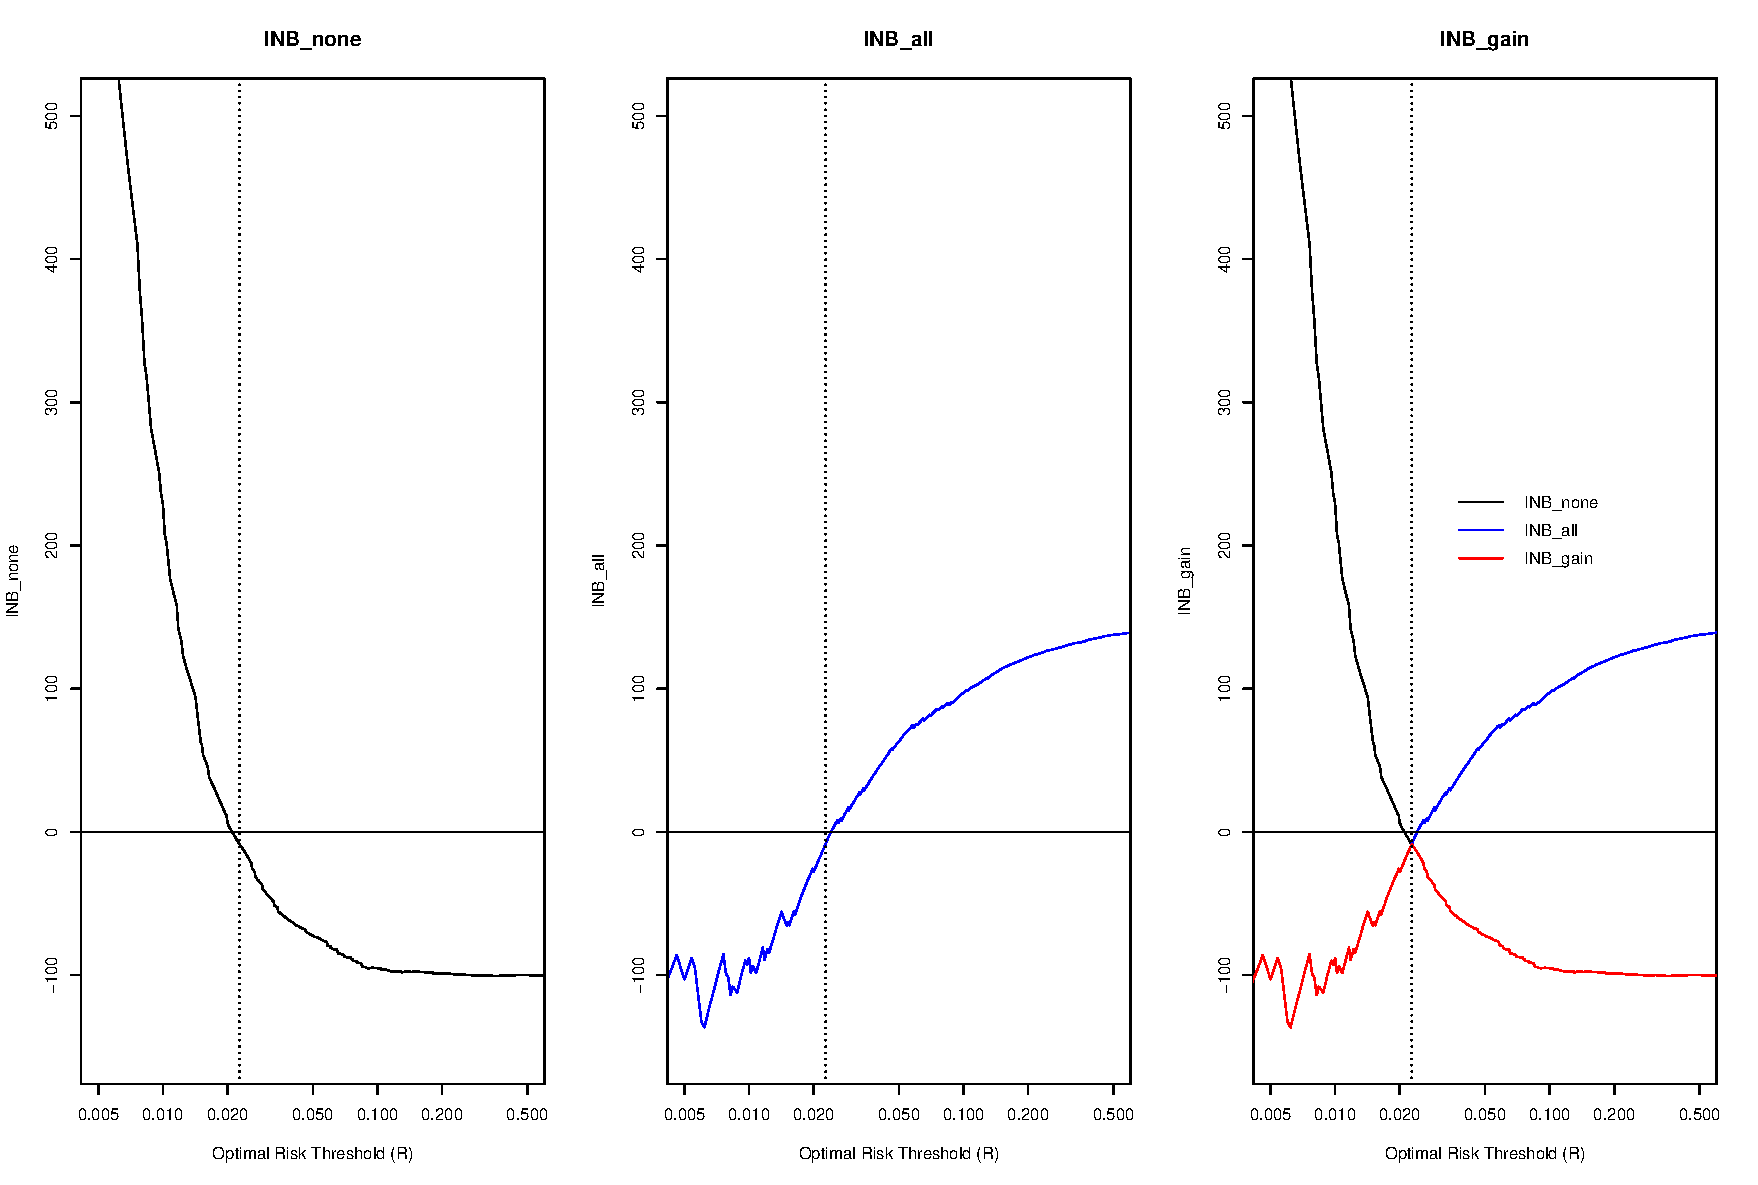
\includegraphics[angle=-0,width=6.5in,]{INBnonevsINBallvsINBgain.pdf}
	\caption{Left panel is Incremental Net Benefit of screening vs testing no one ($I\!N\!B_{none}$).  Thresholds where $I\!N\!B_{none}>0$ favor screening versus testing no one.  Middle panel is Incremental Net Benefit of screening vs testing everyone ($I\!N\!B_{all}$).  Thresholds where $I\!N\!B_{all}>0$ favor screening versus testing everyone.  Right panel is plots both $I\!N\!B_{none}$ and $I\!N\!B_{all}$, highlighting in red the part of each that is $I\!N\!B_{Gain}=min(I\!N\!B_{none},I\!N\!B_{all})$. The vertical line is where the optimal risk threshold equals disease prevalence, which is where $I\!N\!B_{Gain}$ switches over from being equal to $I\!N\!B_{all}$ to being equal to $I\!N\!B_{none}$.  The $I\!N\!B_{Gain}$ equals that of Figure~1 (right panel) of the article.}
	\label{fig:INBnonevsINBallvsINBgain}
\end{figure}



% This section is correct, but leave it out of this paper
%\section{Equivalent specificity condition for a test to have greater INB}
%\label{sec:SpecMoreINB}
%
%The inequality condition for a test having greater INB was written in terms of specificity (equation~\ref{eq:SensMoreINB}).  It  can be equivalently written in terms of specificity: the new marker has better specificity rather than sensitivity.  To see this clearly, we write the above condition in terms of specificity by noting that $P(D+,M+)=P(M+)-P(D-,M+)=p-cSpec\cdot(1-\pi)$ (denoting $cSpec=1-Spec$):
%\begin{eqnarray*}
%	\Delta INB &=& (e+c_0)[p_1-cSpec_1\cdot(1-\pi) - p_2+cSpec_2\cdot(1-\pi)] - c_0[p_1-p_2]\\
%	&=& e[p_1-p_2] +  (e+c_0)(1-\pi)[cSpec_2-cSpec_1]\\
%	&=& e[(1-p_2)-(1-p_1)] + (e+c_0)(1-\pi)[Spec_1-Spec_2] >0
%\end{eqnarray*}
%and presuming $1-p_1>1-p_2$ (so that the sign flips in the inequality),
%\begin{eqnarray*}
%	\frac{Spec_1-Spec_2}{(1-p_1)-(1-p_2)} &>& \frac{e/[e+c_0]}{1-\pi} = \frac{1-\pi_{INB}}{1-\pi}.
%\end{eqnarray*}
%The inequalities based on sensitivity or specificity are equivalent, either can be used.  

%\section{Dollars per life-year gained for one test to be better than another}
%\label{sec:DollarsPerLYGbetterThanAnotherTest}
%We rewrite the key condition involving unequal test costs from section~\ref{sec:moreINB} as 
%\begin{eqnarray*}
%	\frac{\pi[Sens_1-Sens_2]}{ [p_1-p_2] + \frac{c_{m1}-c_{m2}}{c_0}}  &>& R ,
%\end{eqnarray*}
%Denoting the left side of this expression as $s$, we can substitute $s$ for $R$ in the equation for minimum dollars per life-year gained based on optimal threshold $R$ in equation~\ref{eq:dollarsperLYG}, so that we have
%\begin{eqnarray*}
%d = \frac{c_0(1-s)/s + (c_1-c_2)}{e_1-e_2}.
%\end{eqnarray*}


%\section{Bounds on net effectiveness so that screening is better than screening no one or testing everyone}
%\label{sec:BoundsOnNetEffectiveness}
%
%For screening to be cost-effective versus screening no one, then $INB>0$, which happens only if
%\begin{eqnarray*}
%	e &>& \frac{c_m+c_0P(M+)}{P(D+,M+)} - c_0 = \frac{1}{PPV}\left[\frac{c_m}{P(M+)}+c_0(1-PPV)\right]. 
%\end{eqnarray*}
%The minimal net effectiveness is zero only if the marker cost $c_m$ and definitive test cost $c_0$ are zero, else is a positive number.  The minimal net effectiveness required increases with screening-positivity, but decreases with PPV.  If the screening test were free so $c_m=0$ (e.g the screening test were a risk-model based on easily elicited risk factors), then only PPV matters.  This expression holds for any threshold, including the optimal $\pi_{INB}$.
%
%For screening to be better than testing everyone, we need $INB>(e+c_0)P(D+)-c_0$:
%\begin{eqnarray*}
%	0 &<& [e+c_0]P(D+,M+) - c_m - c_0P(M+) - [(e+c_0)P(D+)-c_0] \\
%	0 &<&-[e+c_0]P(D+,M-) - c_m + c_0P(M-) \\
%	e &<& \frac{c_0P(M-)-c_m}{P(D+,M-)} - c_0 = \frac{1}{1-NPV}\left[c_0\cdot NPV - \frac{c_m}{P(M-)}\right]. 
%\end{eqnarray*}
%Note that this is an upper-bound on net effectiveness $e$.  What this means is, if early treatment is too cheap and effective, then just test everyone.
%
%Thus for screening to be better than screening no one or testing everyone, the net effectiveness must be bounded:
%\begin{eqnarray*}
%	\frac{1}{PPV}\left[\frac{c_m}{P(M+)}+c_0(1-PPV)\right] < e < \frac{1}{1-NPV}\left[c_0\cdot NPV - \frac{c_m}{P(M-)}\right]. 
%\end{eqnarray*}
%
%\section{When is INB proportional to MRS, so they have the same maximum?}
%\label{sec:INBandMRS}
%
%Define $p=P(M+)$ and $\pi=P(D+)$.  Recall that $P(D+,M+) = MRS/2 +p\pi$.  Define the net effectiveness of early intervention: $e = (e_1-e_2)-(c_1-c_2)$.  Then
%\begin{eqnarray*}
%	INB &=& (e+c_0)[MRS/2 + p\pi] - c_m - c_0p \\
%	&=& (e+c_0)MRS/2 - c_m + p[e\pi + c_0\pi - c_0] \\
%	&=& (e+c_0)MRS/2 - c_m + p[e\pi - c_0(1-\pi)].
%\end{eqnarray*}
%Note that $INB\propto MRS$ if $e\pi - c_0(1-\pi)=0$, which happens when
%\begin{eqnarray*}
%	\frac{\pi}{1-\pi} &=& \frac{c_0}{e} = \frac{c_0}{(e_1-e_2)-(c_1-c_2)},~~or~~\pi_{INB}=\frac{c_0}{c_0+e}.
%\end{eqnarray*}
%INB and MRS will have the same maximum if the odds of disease equals the ratio of confirmatory test cost to the net effectiveness of early intervention.  Let us call this critical prevalence $\pi_{INB}$ to indicate that this is the disease prevalence where MRS and INB yield the same optimal threshold.  In Figure 1, $c_0/e = \$1,000/(\$400,000-\$0) = 0.25\%$, and thus the critical prevalence is $\pi_{INB}=0.25\%$.  For the general population, $\pi=0.26\%$, which is very close to the critical prevalence.  

%There is no reason for the confirmatory test cost and net effectiveness to balance in a way that their ratio equals the prevalence odds.  However, it is useful to calculate the critical prevalence and compare to the observed disease prevalence, to qualitatively understand which way the threshold for maximum MRS changes when costs and effectiveness are accounted for.  For example, for Ashkenazi-Jews, the prevalence is much higher than the critical prevalence ($2.5\% > 0.25\%$).  Thus immediately you know that the optimal threshold will decrease from prevalence towards testing more women than MRS would indicate.  


%\begin{thebibliography}{}
%	
%	\bibitem[\protect\citeauthoryear{Manchanda}{Manchanda et~al.}{2015}]{Manchanda2015}
%	Manchanda, R., Legood R, Burnell M, McGuire A , et. al.  (2015, July)
%	\newblock Cost-effectiveness of population screening for {BRCA} mutations in {A}shkenazi jewish women compared with family history-based testing.
%	\newblock {\em J Natl Cancer Inst\/}~{\em 107(1)}, 380.
%	
%\end{thebibliography}


\end{document}
% ------------------------------------------------------------------------
